\documentclass[11pt]{article}
\usepackage[margin=1in]{geometry}
\usepackage{graphicx}
\usepackage{amsmath}
\usepackage{booktabs}
\usepackage{float}
\usepackage{hyperref}

\title{Experiment 25}
\author{Ansh Tiwari}
\date{\today}

\begin{document}
\maketitle

\section{Post Lab Analysis}

\subsection{Theory}

This experiment uses the isotope shift between hydrogen and deuterium Balmer lines to estimate the proton electron mass ratio. The energy levels of a hydrogen like atom depend on the reduced mass of the electron nucleus system,

\[
\mu = \frac{m_e m_N}{m_e + m_N}.
\]

Hydrogen has a proton as its nucleus. Deuterium has a heavier nucleus made from a proton and a neutron. The deuterium reduced mass is therefore slightly larger than the hydrogen reduced mass. Since the transition energy is proportional to the reduced mass, the deuterium transition energy is slightly larger, so the deuterium line appears at a slightly shorter wavelength.

The measured isotope shift is

\[
\Delta \lambda = \lambda_{\mathrm{H}} - \lambda_{\mathrm{D}}.
\]

For corresponding Balmer transitions, the expected relation is

\[
\Delta \lambda
\approx
0.500 \frac{m_e}{m_p} \lambda_{\mathrm{H}}.
\]

I write this as

\[
\Delta \lambda = s \lambda_{\mathrm{H}}.
\]

The proton electron mass ratio is then

\[
\frac{m_p}{m_e} = \frac{0.500}{s}.
\]

The analysis therefore has three main parts. First, the monochromator wavelength scale is calibrated with mercury lines. Second, the hydrogen and deuterium peaks are identified and fit. Third, the isotope shift relation is used to estimate \(m_p/m_e\).

\subsection{Preparation}

All scans were first converted from the second order instrument setting to the real wavelength scale using

\[
\lambda_{\mathrm{real}} = \frac{\lambda_{\mathrm{instrument}}}{2}.
\]

The raw data were kept unchanged, and separate real wavelength files were made for fitting. The files were classified as mercury calibration scans, hydrogen only control scans, and hydrogen deuterium mixed lamp scans.

The CurveFit package was used to make reference plots and appendix reports because it was part of the lab workflow. The main numerical analysis used Mathematica's built in fitting functions. This made it possible to control the fit window, model form, parameter constraints, residuals, and uncertainty propagation directly.

\subsection{Calibration}

The mercury peaks were fit with a Gaussian peak plus a linear background,

\[
V(\lambda)
=
c + d(\lambda - \lambda_0)
+
A \exp\left[-\frac{(\lambda - \mu)^2}{2\sigma^2}\right].
\]

The fitted center \(\mu\) was treated as the observed mercury wavelength. The main calibration used the 365.588 nm, 404.770 nm, and 546.226 nm mercury lines. The 365.119 nm region was fit as a diagnostic but was not used as a main calibration point because the 365 nm region contains nearby mercury lines, and the fitted center was not independent of the 365.588 nm fit.

The calibration model was

\[
\lambda_{\mathrm{true}} = a + b\lambda_{\mathrm{obs}}.
\]

The fit gave

\[
a = 0.423 \pm 0.738 \ \mathrm{nm},
\]

\[
b = 0.998274 \pm 0.001655.
\]

The root mean square calibration residual was

\[
0.129 \ \mathrm{nm},
\]

and the maximum absolute residual was

\[
0.173 \ \mathrm{nm}.
\]

Figure~\ref{fig:hgcal} shows the calibration and residuals. The calibration residuals are not zero, so the wavelength calibration is not perfect. However, the intercept \(a\) cancels in a hydrogen deuterium pair separation. For two peaks measured in the same scan,

\[
\lambda_{\mathrm{H,corr}} = a + b\mu_{\mathrm{H}},
\]

\[
\lambda_{\mathrm{D,corr}} = a + b\mu_{\mathrm{D}},
\]

so

\[
\Delta \lambda_{\mathrm{corr}}
=
\lambda_{\mathrm{H,corr}} - \lambda_{\mathrm{D,corr}}
=
b(\mu_{\mathrm{H}} - \mu_{\mathrm{D}}).
\]

This means the calibration slope \(b\) directly affects the measured isotope shift, while the intercept mainly affects the absolute wavelength positions.

\begin{figure}[htbp]
\centering
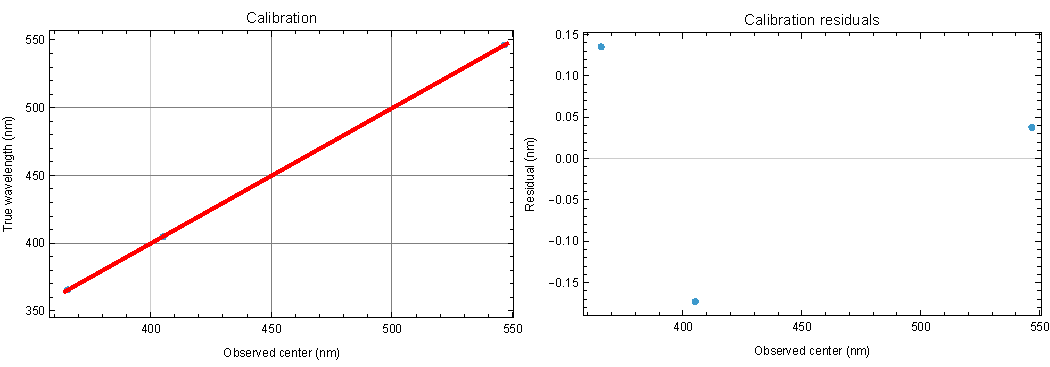
\includegraphics[width=0.82\textwidth]{PHASE1_real_wavelength_files/PHASE2_Hg_calibration_native_clean/compact_calibration_figures/Hg_calibration_and_residuals_compact.pdf}
\caption{Mercury wavelength calibration and residuals. The calibration maps fitted mercury centers to true mercury vacuum wavelengths.}
\label{fig:hgcal}
\end{figure}

\begin{table}[htbp]
\centering
\caption{Mercury peak fits used to evaluate the wavelength calibration and line width.}
\label{tab:hgfits}
\begin{tabular}{lrrrrr}
\hline
Line & True nm & Observed nm & Center error nm & Width nm & Used \\
\hline
Hg 365.119 diagnostic & 365.119 & 365.662 & 0.00112 & 0.06798 & no \\
Hg 365.588 & 365.588 & 365.660 & 0.00206 & 0.07343 & yes \\
Hg 404.770 & 404.770 & 405.219 & 0.00112 & 0.06138 & yes \\
Hg 546.226 & 546.226 & 546.708 & 0.00079 & 0.06990 & yes \\
Hg 546 repeat wide & 546.226 & 546.694 & 0.00097 & 0.07592 & no \\
Hg 546 repeat 20um & 546.226 & 546.680 & 0.00202 & 0.07805 & no \\
\hline
\end{tabular}
\end{table}

\subsection{Resolution}

The fitted mercury widths estimate the instrumental width of a single spectral line. I converted each Gaussian width to a full width using

\[
\mathrm{FWHM} = 2\sqrt{2\ln2}\sigma.
\]

The mercury full widths were about \(0.14\) nm to \(0.18\) nm. This is comparable to the expected hydrogen and deuterium separation. Therefore, the hydrogen and deuterium peaks are not completely separated. This is why the final analysis uses peak models rather than simply reading off two maximum positions.

\begin{figure}[htbp]
\centering
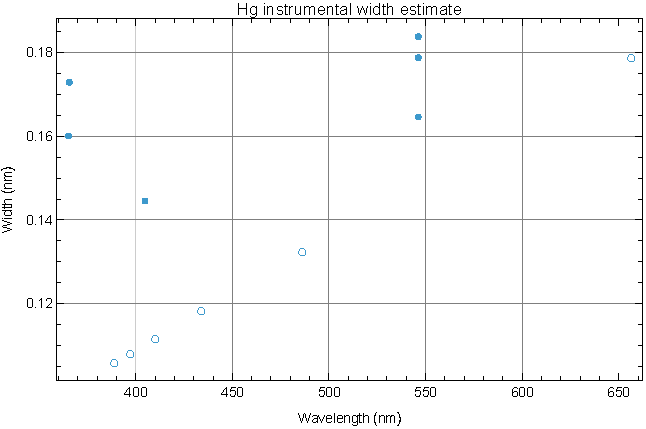
\includegraphics[width=0.55\textwidth]{PHASE1_real_wavelength_files/PHASE3_instrument_resolution/Hg_FWHM_vs_HD_separation_scale.pdf}
\caption{Instrumental width estimated from mercury fits. The line widths are comparable to the isotope shift scale, so peak overlap matters.}
\label{fig:widths}
\end{figure}

\begin{table}[htbp]
\centering
\caption{Instrumental width estimates from mercury fits.}
\label{tab:widths}
\begin{tabular}{lrrrrr}
\hline
Line & True nm & \(\sigma\) nm & FWHM nm & Residual V & Used \\
\hline
Hg 365.119 diagnostic & 365.119 & 0.0680 & 0.1601 & 0.2298 & False \\
Hg 365.588 & 365.588 & 0.0734 & 0.1729 & 0.1920 & True \\
Hg 404.770 & 404.770 & 0.0614 & 0.1445 & 0.1473 & True \\
Hg 546.226 & 546.226 & 0.0699 & 0.1646 & 0.0273 & True \\
Hg 546 repeat wide & 546.226 & 0.0759 & 0.1788 & 0.0459 & False \\
Hg 546 repeat 20um & 546.226 & 0.0781 & 0.1838 & 0.0636 & False \\\hline%
\end{tabular}
\end{table}

\subsection{Controls}

The hydrogen only spectra were used as controls. The purpose was to see what a single hydrogen line looked like with the same instrument and to identify regions where other spectral features were present. Several hydrogen only lines were well described by a single Gaussian plus a linear background. H epsilon and H zeta were not clean single peak spectra. They showed extra structure that could not be honestly absorbed into a straight background.

Figure~\ref{fig:hcontrol} summarizes the single peak hydrogen only fits. The large residuals for some lines show that not every region of the spectrum is clean.

\begin{figure}[htbp]
\centering
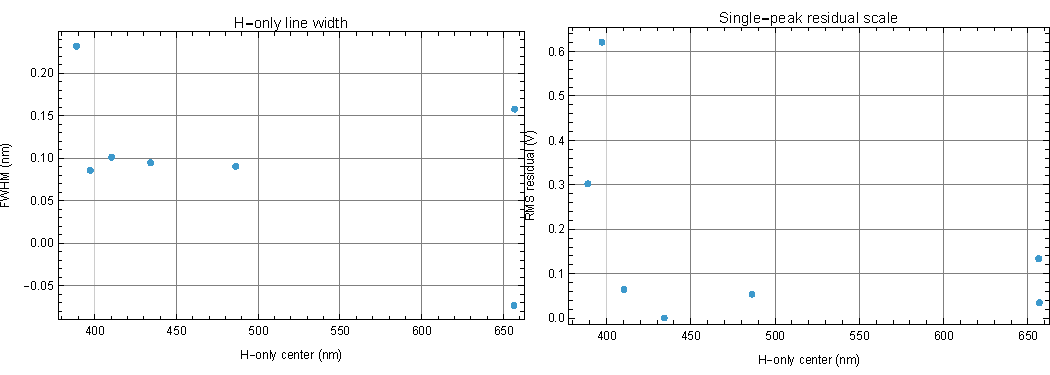
\includegraphics[width=0.62\textwidth]{PHASE1_real_wavelength_files/PHASE4_Hydrogen_only_control/hydrogen_only_width_and_residual_summary.pdf}
\caption{Hydrogen only single peak fit summary. Left: fitted Gaussian FWHM versus line center. Right: single peak RMS residual versus line center. H epsilon and H zeta have larger residuals because of extra structure in those regions.}
\label{fig:hcontrol}
\end{figure}

\begin{table}[htbp]
\centering
\caption{Hydrogen only single peak fit results.}
\label{tab:hcontrol}
\begin{tabular}{lrrrrr}
\hline
Line & Center nm & Center error nm & \(\sigma\) nm & FWHM nm & Residual V \\
\hline
H alpha & 656.401 & 0.00030 & -0.0311 & -0.0732 & 0.1339 \\
H alpha & 656.835 & 0.00062 & 0.0669 & 0.1575 & 0.0350 \\
H zeta & 388.889 & 0.00591 & 0.0984 & 0.2316 & 0.3021 \\
H epsilon & 397.285 & 0.00435 & 0.0363 & 0.0855 & 0.6210 \\
H delta & 410.383 & 0.00027 & 0.0429 & 0.1010 & 0.0647 \\
H gamma & 434.251 & 0.00022 & 0.0401 & 0.0944 & 0.0005 \\
H beta & 486.308 & 0.00026 & 0.0383 & 0.0902 & 0.0539 \\\hline%
\end{tabular}
\end{table}

For H epsilon and H zeta, I also tried two Gaussian models. These models showed that the extra structure could be described empirically, but the interpretation was not clean enough to use those lines in the main isotope shift fit. The line identity maps also supported this decision. The zeta region overlapped with possible first order oxygen features near 777 nm after second order conversion, and the epsilon region showed several extra peaks in both the hydrogen only and mixed lamp scans.

\subsection{Peak Fits}

The first main hydrogen deuterium peak model was a two peak Gaussian model with a shared width and a linear background,

\[
V(\lambda)
=
c + d(\lambda - \lambda_0)
+
A_{\mathrm{D}}\exp\left[-\frac{(\lambda-\mu_{\mathrm{D}})^2}{2\sigma^2}\right]
+
A_{\mathrm{H}}\exp\left[-\frac{(\lambda-\mu_{\mathrm{H}})^2}{2\sigma^2}\right].
\]

The shorter wavelength peak was assigned to deuterium, and the longer wavelength peak was assigned to hydrogen. This follows from the reduced mass argument because deuterium has the shorter wavelength.

The observed separation was

\[
\Delta\lambda_{\mathrm{obs}} = \mu_{\mathrm{H}} - \mu_{\mathrm{D}}.
\]

The corrected separation was

\[
\Delta\lambda_{\mathrm{corr}} = b\Delta\lambda_{\mathrm{obs}}.
\]

The uncertainty was propagated as

\[
\sigma_{\Delta,\mathrm{corr}}
=
\sqrt{
(b\sigma_{\Delta,\mathrm{obs}})^2
+
(\Delta\lambda_{\mathrm{obs}}\sigma_b)^2
}.
\]

H beta, H gamma, and H delta were fit with constrained shared width models. H alpha needed special treatment. The global two peak fit did not properly model the visible hydrogen peak, so I fit the deuterium and hydrogen peaks in separate local windows. The local H alpha fits are shown in Fig.~\ref{fig:halpha}.

\begin{figure}[htbp]
\centering
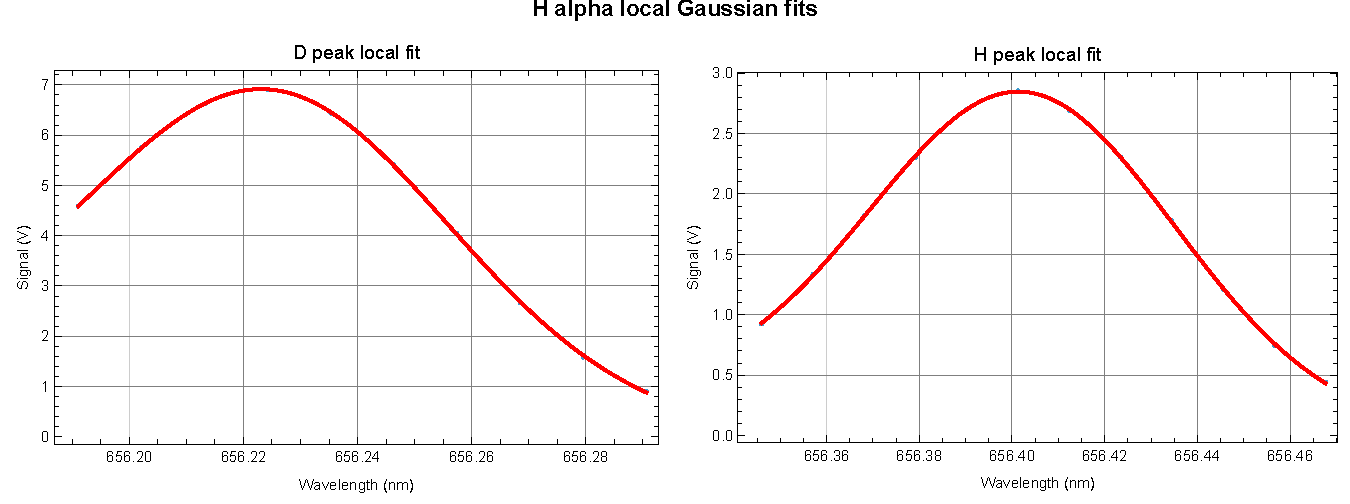
\includegraphics[width=0.47\textwidth]{PHASE1_real_wavelength_files/PHASE5D_H_alpha_local_refit/H_alpha_local_refit_fit_row.pdf}
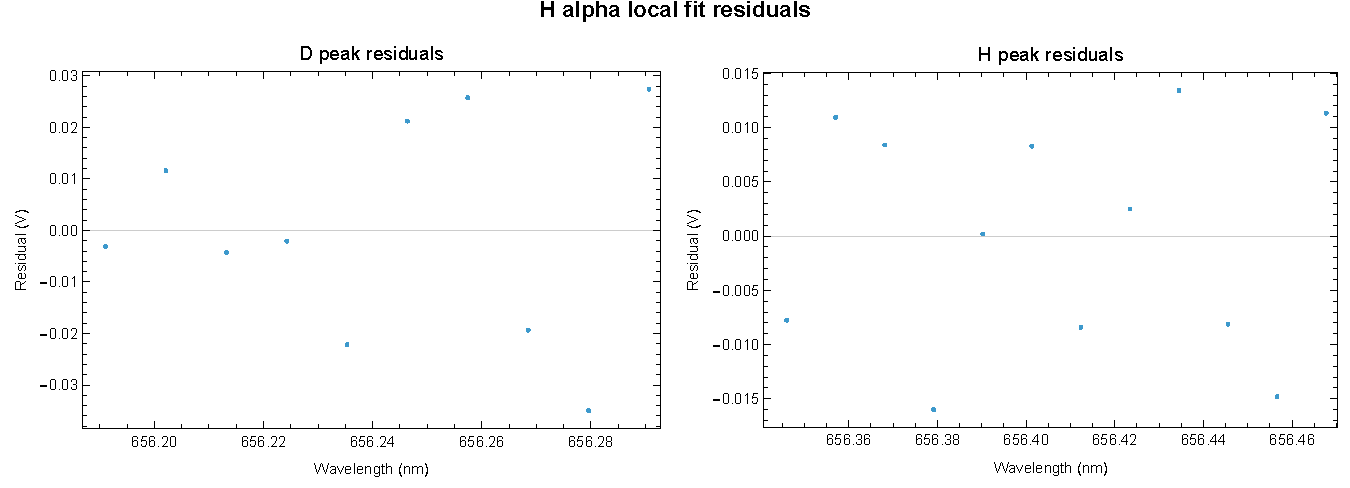
\includegraphics[width=0.47\textwidth]{PHASE1_real_wavelength_files/PHASE5D_H_alpha_local_refit/H_alpha_local_refit_residual_row.pdf}
\caption{Local H alpha refit. The deuterium peak and hydrogen peak were fit in separate windows because the global two peak model did not fit the right peak well.}
\label{fig:halpha}
\end{figure}

The separate peak fits gave a first full estimate of the mass ratio. This was useful because it showed that the corrected separations increased with hydrogen wavelength, as expected. However, this approach first extracts the separations and then fits the isotope shift relation. I later used a more direct global fit where the isotope shift relation was built into the spectral model itself.

\begin{table}[htbp]
\centering
\caption{Corrected hydrogen wavelengths and corrected isotope shifts from the separate peak analysis.}
\label{tab:fitpoints}
\begin{tabular}{lrrrl}
\hline
Line & \(\lambda_{\mathrm{H,corr}}\) nm & \(\Delta\lambda_{\mathrm{corr}}\) nm & Error nm & Source \\
\hline
H delta & 410.1280 & 0.10909 & 0.00099 & shared width fit \\
H gamma & 433.9560 & 0.11155 & 0.00070 & shared width fit \\
H beta & 485.9120 & 0.13329 & 0.00037 & shared width fit \\
H alpha & 655.6930 & 0.17726 & 0.00066 & local refit \\
\hline
\end{tabular}
\end{table}

\subsection{Global Fit}

The final analysis used a global physics constrained fit. In this fit, the isotope shift relation was built directly into the peak model. Instead of measuring four separations first and then fitting a line, the spectra were fit together using one shared isotope shift slope \(s\).

For each line, the hydrogen center was allowed to vary, but the deuterium center was constrained by the relation

\[
\Delta \lambda_{\mathrm{corr}} = s\lambda_{\mathrm{H,corr}}.
\]

Using the calibration equation

\[
\lambda_{\mathrm{corr}} = a + b\lambda_{\mathrm{obs}},
\]

this means the deuterium center in observed wavelength units is

\[
\mu_{\mathrm{D}}
=
\mu_{\mathrm{H}}
-
\frac{s}{b}
\left(a+b\mu_{\mathrm{H}}\right).
\]

The fit used H alpha, H beta, H gamma, and H delta. H epsilon and H zeta were excluded because they were not clean hydrogen deuterium doublets. The nuisance parameters were the peak heights, the local backgrounds, the widths, and the hydrogen centers. The shared physical parameter was \(s\).

The global constrained fit gave

\[
s = 2.71553\times 10^{-4}.
\]

Therefore,

\[
\frac{m_p}{m_e}
=
\frac{0.500}{s}
=
1841.26.
\]

The residual root mean square over all spectral points was

\[
0.02685 \ \mathrm{V}.
\]

This residual is in detector voltage because the fit was done directly on the spectra.

\begin{figure}[htbp]
\centering
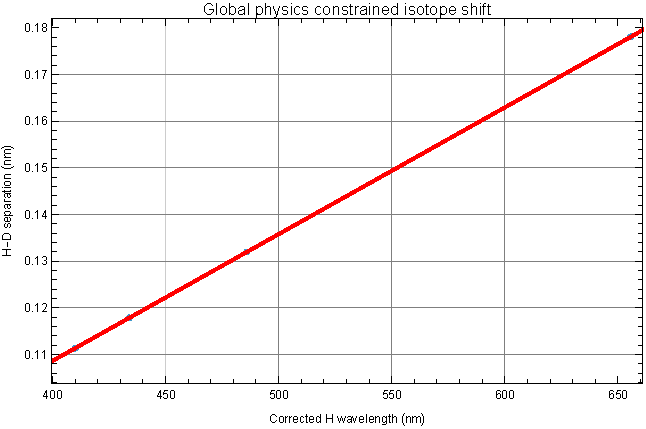
\includegraphics[width=0.62\textwidth]{PHASE1_real_wavelength_files/PHASE10_global_physics_constrained_fit/figures/global_physics_constrained_shift_fit.pdf}
\caption{Hydrogen deuterium separations implied by the global physics constrained fit. The red line is the shared isotope shift relation used inside the spectral fit.}
\label{fig:globalshift}
\end{figure}

\begin{table}[htbp]
\centering
\caption{Line centers from the global physics constrained fit.}
\label{tab:globalfit}
\begin{tabular}{lrrrrrr}
\hline
Line & \(\mu_D\) & \(\mu_H\) & \(\Delta\lambda\) & \(\lambda_H\) & \(\Delta\lambda_c\) & \(\sigma\) \\
\hline
H alpha & 656.2223 & 656.4006 & 0.17836 & 655.6911 & 0.17806 & 0.0328 \\
H beta & 486.1944 & 486.3266 & 0.13218 & 485.9106 & 0.13195 & 0.0399 \\
H gamma & 434.1700 & 434.2880 & 0.11805 & 433.9619 & 0.11784 & 0.0316 \\
H delta & 410.3028 & 410.4143 & 0.11156 & 410.1294 & 0.11137 & 0.0419 \\
\end{tabular}
\end{table}

\subsection{Profile Error}

The covariance matrix did not give a reliable uncertainty for the global slope because the model was nonlinear and used bounded transformed parameters. I therefore estimated the uncertainty with a profile scan.

In the profile scan, I fixed the slope \(s\) at many values near the best fit. For each fixed value of \(s\), all nuisance parameters were refit. These nuisance parameters included peak heights, widths, center positions allowed by the constraint, and local backgrounds. Then I recorded the total residual sum of squares,

\[
RSS(s)-RSS_{\min}.
\]

The profile best value matched the global fit,

\[
s = 2.71553\times 10^{-4},
\]

which gives

\[
m_p/m_e = 1841.26.
\]

The one sigma profile interval was

\[
1839.71 \leq m_p/m_e \leq 1842.83.
\]

So the profile result is

\[
\frac{m_p}{m_e}
=
1841.3^{+1.6}_{-1.5}.
\]

The two sigma profile interval was

\[
1835.08 \leq m_p/m_e \leq 1847.58.
\]

This interval includes the expected value near \(1836\). The profile uncertainty is the uncertainty inside the chosen global model. It does not include all possible systematic uncertainty from model choice, fit windows, and spectral contamination.

\begin{figure}[htbp]
\centering
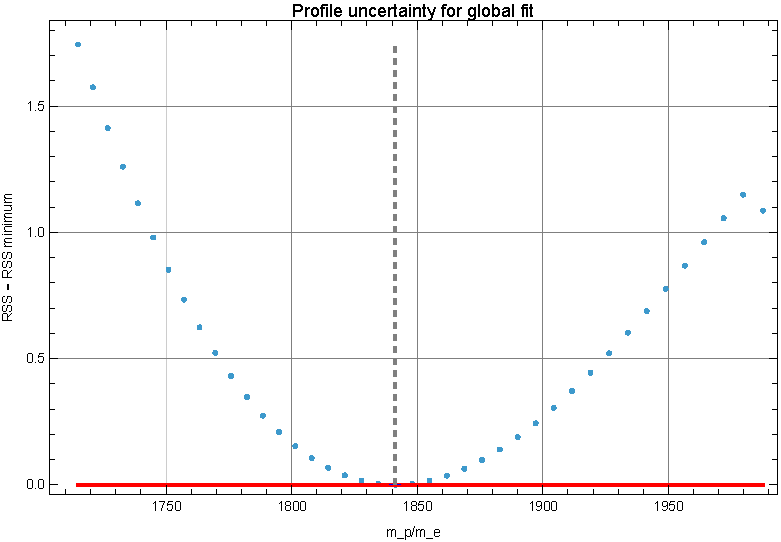
\includegraphics[width=0.58\textwidth]{PHASE1_real_wavelength_files/PHASE10B_global_profile_uncertainty/figures/global_profile_uncertainty_curve.pdf}
\caption{Profile uncertainty curve for the global constrained fit. The slope was fixed at different values, while all nuisance fit parameters were refit.}
\label{fig:profile}
\end{figure}

\begin{table}[htbp]
\centering
\caption{Profile uncertainty result for the global constrained fit.}
\label{tab:profile}
\begin{tabular}{lr}
\hline
Quantity & Value \\
\hline
Global slope $s$ & 0.0002716 \\
$m_p/m_e$ & 1841.3$^{+1.6}_{-1.5}$ \\
RSS minimum & 0.07642 \\
Degrees of freedom & 81 \\\hline%
\end{tabular}
\end{table}

\subsection{Model Checks}

I checked whether the final result depended strongly on the assumed line shape. The first peak fits used Gaussian peaks. As a second model, I used the measured Hg 546 nm line as an empirical instrument response. In that model, the peak shape was not assumed to be a perfect Gaussian. Instead, the measured response shape \(R\) from mercury was used as the peak template,

\[
V(\lambda)
=
A_D R(\lambda-\lambda_D)
+
A_H R(\lambda-\lambda_H)
+
\text{background}.
\]

This model worked well for clean doublets like H beta and H gamma. It also gave a reasonable diagnostic fit for H delta. A global empirical response fit for H alpha did not work well, because the separation hit the allowed upper bound. I then fit H alpha locally with the empirical response shape, which gave a much better local fit.

The model comparison is shown in Table~\ref{tab:modelcompare}. The Gaussian model with local H alpha, the empirical response model without H alpha, and the empirical response model with local H alpha all gave mass ratios near the right scale. However, the empirical response models shifted the final value upward. This shows that line shape choice is a real systematic effect.

\begin{table}[htbp]
\centering
\caption{Model comparison for the final isotope shift fit.}
\label{tab:modelcompare}
\begin{tabular}{lrrrr}
\hline
Model & Points & Slope \(s\) & \(m_p/m_e\) & RMS residual nm \\
\hline
Gaussian with local H alpha & 4 & \(2.68088\times10^{-4}\) & \(1865.1 \pm 23.5\) & 0.00296 \\
Empirical response without H alpha & 3 & \(2.58500\times10^{-4}\) & \(1934.2 \pm 32.8\) & 0.00276 \\
Empirical response with local H alpha & 4 & \(2.63763\times10^{-4}\) & \(1895.6 \pm 32.3\) & 0.00393 \\
\hline
\end{tabular}
\end{table}

The model comparison does not replace the global constrained result. It tells us how much the answer can move when the peak shape model is changed. The global constrained fit is still the best main result because it fits the spectra directly while enforcing the isotope shift relation across all four usable Balmer lines.

\subsection{Derived Values}

Using the global constrained mass ratio and the electron rest energy \(0.511\) MeV, the proton rest energy estimate is

\[
m_p c^2
=
1841.26(0.511 \ \mathrm{MeV})
=
940.68 \ \mathrm{MeV}.
\]

Using the one sigma profile uncertainty,

\[
\sigma_{m_p c^2}
=
1.56(0.511 \ \mathrm{MeV})
\approx
0.80 \ \mathrm{MeV}.
\]

So,

\[
m_p c^2 = 940.7 \pm 0.8 \ \mathrm{MeV}.
\]

Using \(m_e = 9.109\times10^{-31}\) kg, the hydrogen atom mass is approximately

\[
m_{\mathrm{H}}
\approx
(m_p/m_e+1)m_e
=
1.678\times10^{-27} \ \mathrm{kg}.
\]

A hydrogen molecule has two hydrogen atoms, so a \(2\) g mole of hydrogen gas gives

\[
N_A
=
\frac{0.002 \ \mathrm{kg}}{2m_{\mathrm{H}}}
=
5.96\times10^{23}.
\]

The uncertainty from the profile error alone gives

\[
N_A = (5.96 \pm 0.01)\times10^{23}.
\]

This is close to the accepted scale of Avogadro's number. The uncertainty here only includes the profile uncertainty from the spectroscopic fit, not all possible systematic errors.

\subsection{Discussion}

The final global constrained result was

\[
m_p/m_e = 1841.3^{+1.6}_{-1.5}.
\]

This is close to the expected value near \(1836\). The two sigma profile interval includes the expected value. The result is also physically consistent because the measured isotope shift increases with hydrogen wavelength.

The main strength of the global fit is that it uses the isotope shift theory directly while fitting the spectra. Instead of first extracting four independent separations and then fitting a line, the global model forces all four usable spectra to share the same physical slope \(s\). This reduces the freedom of the fit and gives a more direct estimate of the mass ratio.

The profile uncertainty shows that the statistical uncertainty inside the global model is small. However, the model comparison shows that line shape choices can move the answer by a larger amount. For example, using the empirical mercury response instead of Gaussian peaks shifted the mass ratio upward. This means the final result should be interpreted as a precise result within one model, with a larger systematic uncertainty from peak model choice.

The hydrogen only controls and line identity maps showed why H epsilon and H zeta were excluded. Those regions contained extra peaks in both the hydrogen only and mixed lamp scans. The zeta region also overlaps possible first order oxygen aliases. It would not be honest to treat those regions as clean hydrogen deuterium doublets without a more detailed contamination model.

H alpha required special treatment because the global unconstrained two peak fit did not describe the right peak well. Local fitting fixed this issue, and the later global constrained fit gave a value close to the expected mass ratio. This suggests that the main limitation is not the isotope shift relation itself, but how accurately the peak centers can be extracted from overlapping and sometimes contaminated spectral features.

\subsection{Conclusion}

The Balmer isotope shift was measured from hydrogen deuterium spectra and used to estimate the proton electron mass ratio. After mercury calibration, hydrogen only control checks, line identity checks, constrained peak fits, and a global physics constrained fit, the final result was

\[
\boxed{
m_p/m_e = 1841.3^{+1.6}_{-1.5}
}
\]

from the profile uncertainty of the global fit. The result is within about \(0.3\%\) of the expected value and has the expected value inside the two sigma profile interval.

The strongest remaining limitation is model dependence. The profile uncertainty is small, but alternate reasonable line shape models shift the result by more than the profile error. Therefore, the best interpretation is that the experiment successfully measured the isotope shift and obtained the correct proton electron mass ratio scale, with the main systematic uncertainty coming from peak shape, fit window, and spectral contamination choices.

\clearpage
\appendix

\section{Appendix}

\subsection{Mercury Fits}

This appendix contains the mercury fit figures from the native Mathematica analysis. These figures support the calibration values and the instrumental width estimate.

\begin{figure}[H]
\centering
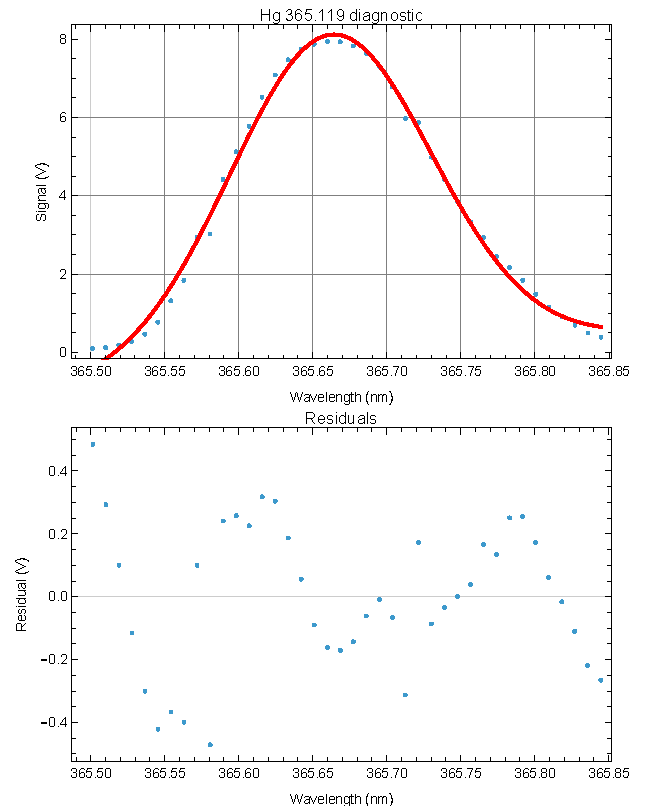
\includegraphics[width=0.48\textwidth]{PHASE1_real_wavelength_files/PHASE2_Hg_calibration_native_clean/fit_figures_no_tables/Hg_365p119_diagnostic_fit_residual_clean.pdf}
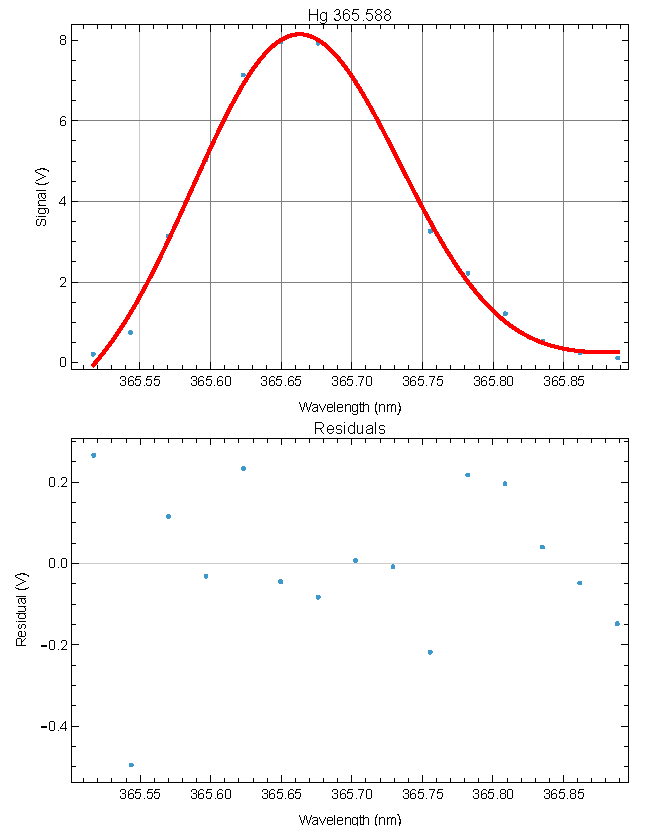
\includegraphics[width=0.48\textwidth]{PHASE1_real_wavelength_files/PHASE2_Hg_calibration_native_clean/fit_figures_no_tables/Hg_365p588_fit_residual_clean.pdf}
\caption{Mercury fits near 365 nm. The first is diagnostic only, and the second was used for calibration.}
\end{figure}

\begin{figure}[H]
\centering
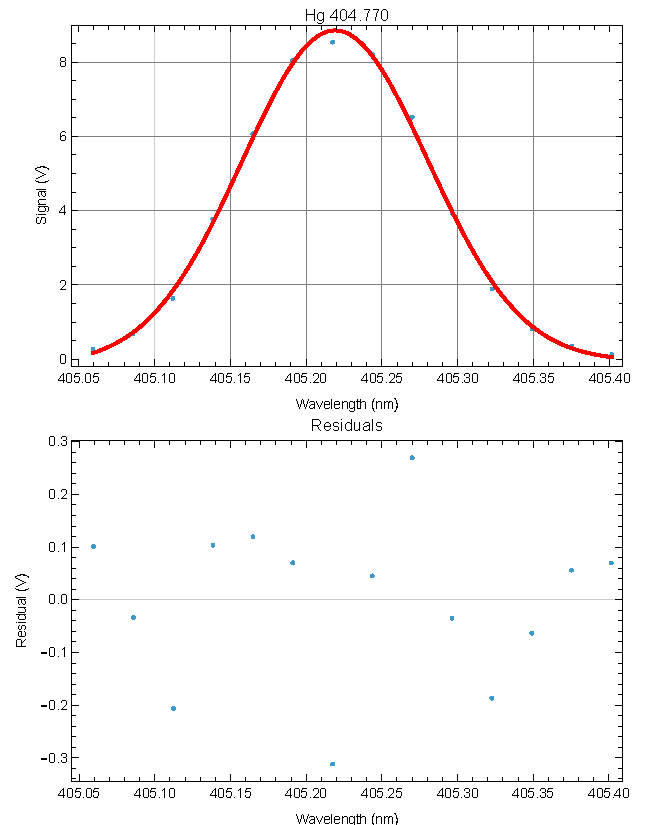
\includegraphics[width=0.48\textwidth]{PHASE1_real_wavelength_files/PHASE2_Hg_calibration_native_clean/fit_figures_no_tables/Hg_404p770_fit_residual_clean.pdf}
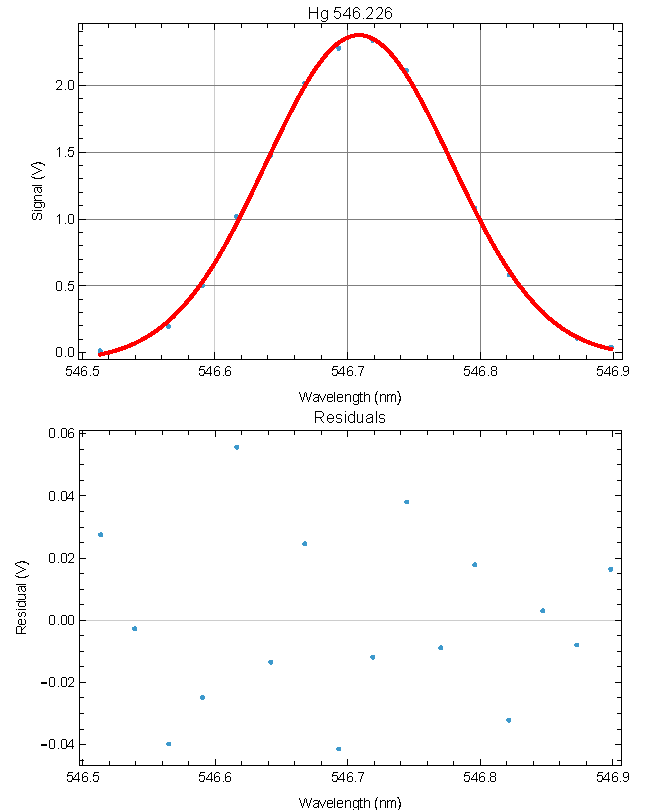
\includegraphics[width=0.48\textwidth]{PHASE1_real_wavelength_files/PHASE2_Hg_calibration_native_clean/fit_figures_no_tables/Hg_546p226_fit_residual_clean.pdf}
\caption{Mercury fits for 404.770 nm and 546.226 nm used in the calibration.}
\end{figure}

\begin{figure}[H]
\centering
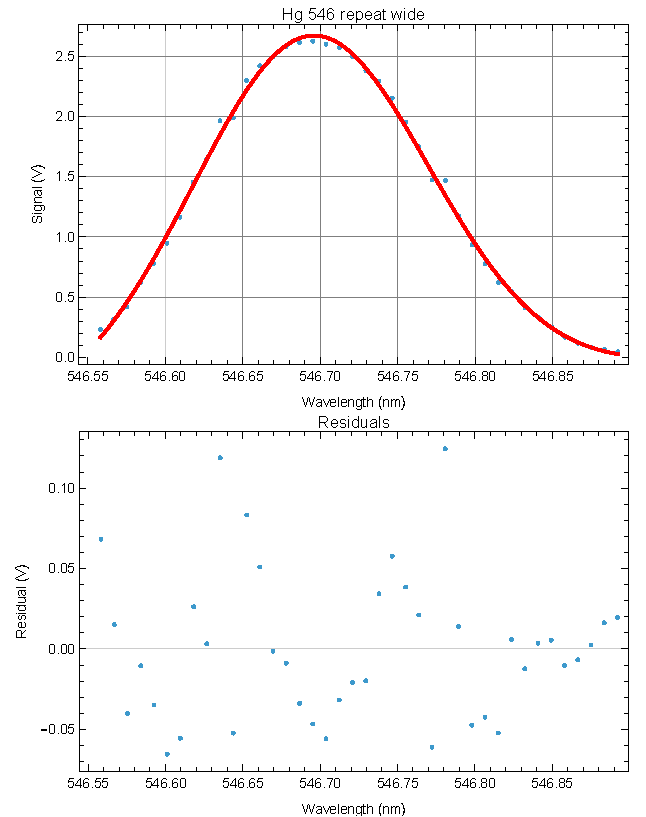
\includegraphics[width=0.48\textwidth]{PHASE1_real_wavelength_files/PHASE2_Hg_calibration_native_clean/fit_figures_no_tables/Hg_546_repeat_wide_fit_residual_clean.pdf}
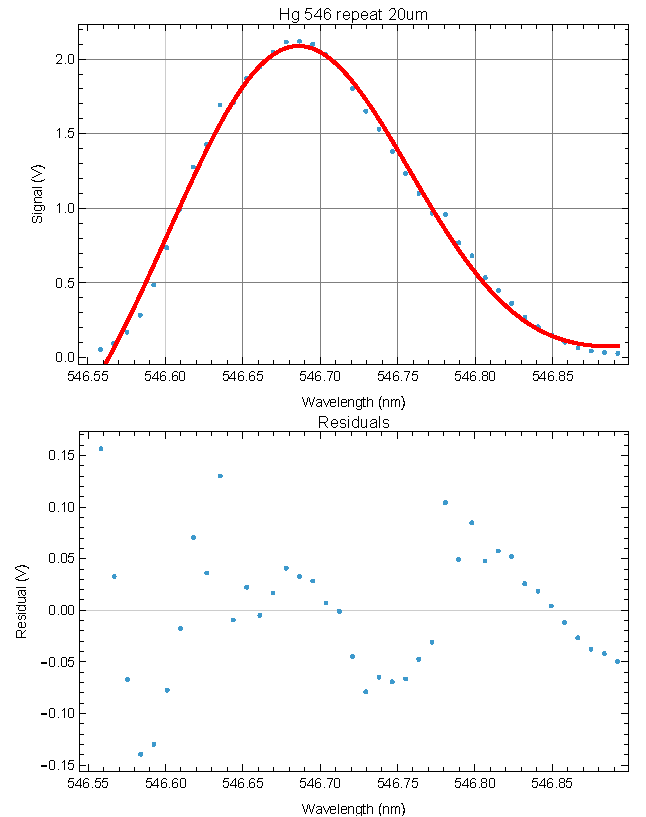
\includegraphics[width=0.48\textwidth]{PHASE1_real_wavelength_files/PHASE2_Hg_calibration_native_clean/fit_figures_no_tables/Hg_546_repeat_20um_fit_residual_clean.pdf}
\caption{Repeated 546 nm mercury fits used as repeatability checks. These were not used as independent calibration lines.}
\end{figure}

\subsection{Control Fits}

The hydrogen only fits were used to identify which spectral regions were clean and which were contaminated by extra structure.

\begin{figure}[H]
\centering
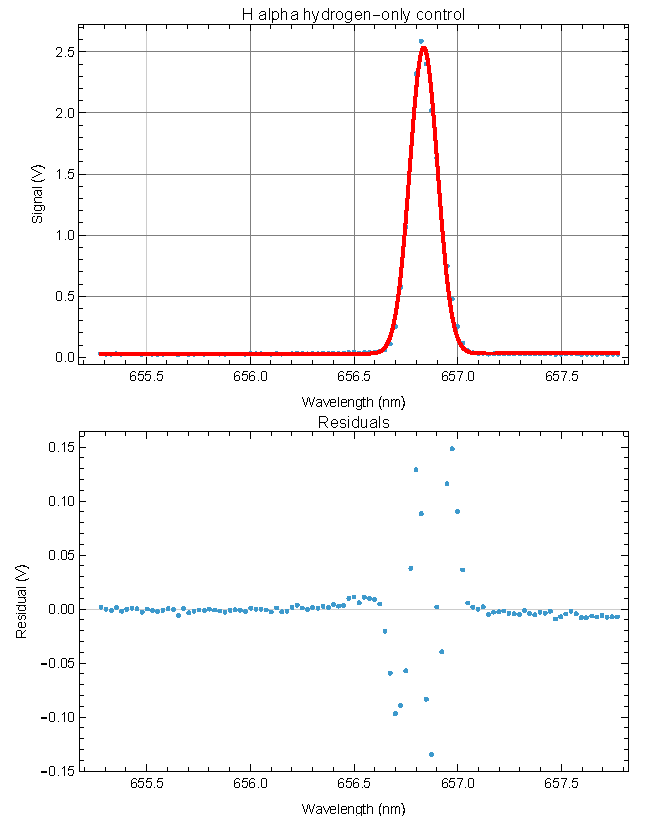
\includegraphics[width=0.48\textwidth]{PHASE1_real_wavelength_files/PHASE4_Hydrogen_only_control/fit_figures_no_tables/H_alpha_hydrogen_only_fit_residual.pdf}
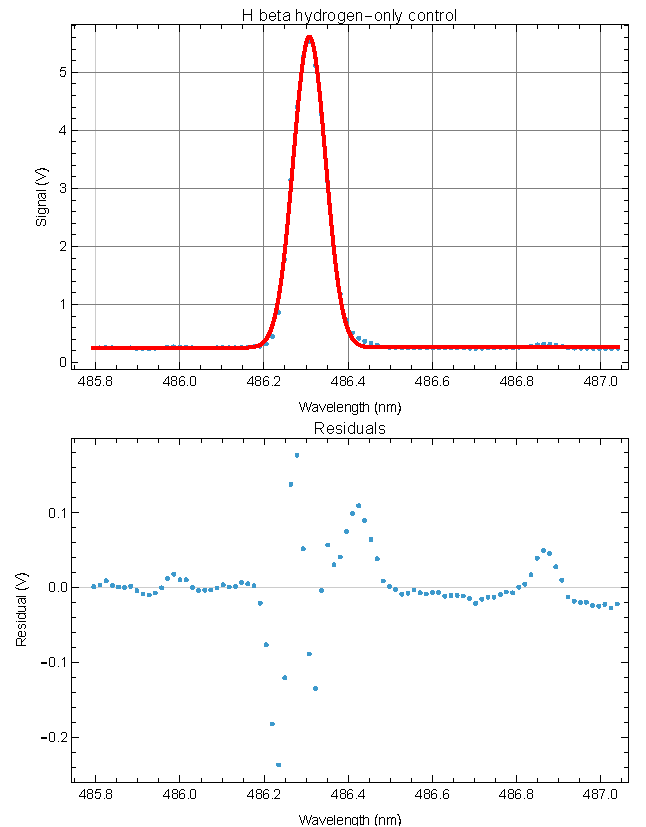
\includegraphics[width=0.48\textwidth]{PHASE1_real_wavelength_files/PHASE4_Hydrogen_only_control/fit_figures_no_tables/H_beta_hydrogen_only_fit_residual.pdf}
\caption{Hydrogen only control fits for H alpha and H beta.}
\end{figure}

\begin{figure}[H]
\centering
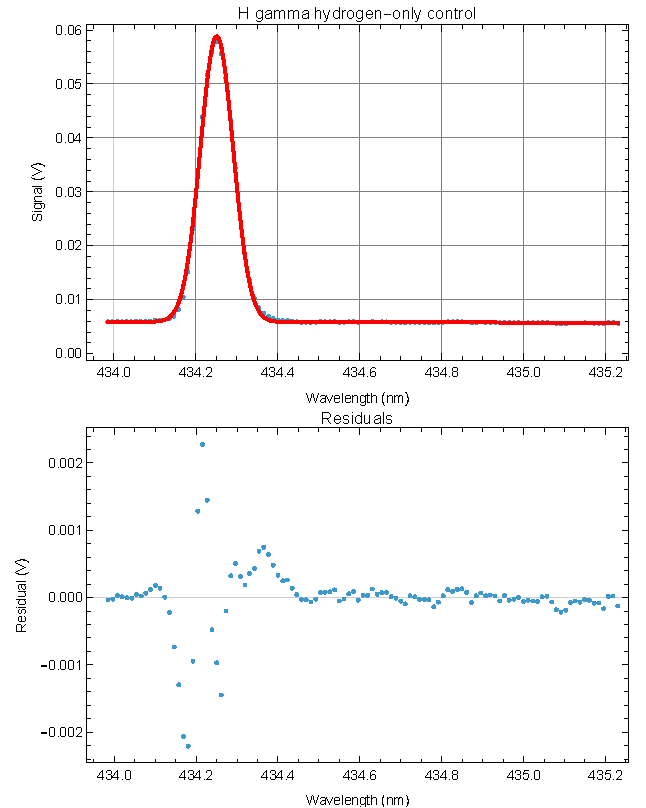
\includegraphics[width=0.48\textwidth]{PHASE1_real_wavelength_files/PHASE4_Hydrogen_only_control/fit_figures_no_tables/H_gamma_hydrogen_only_fit_residual.pdf}
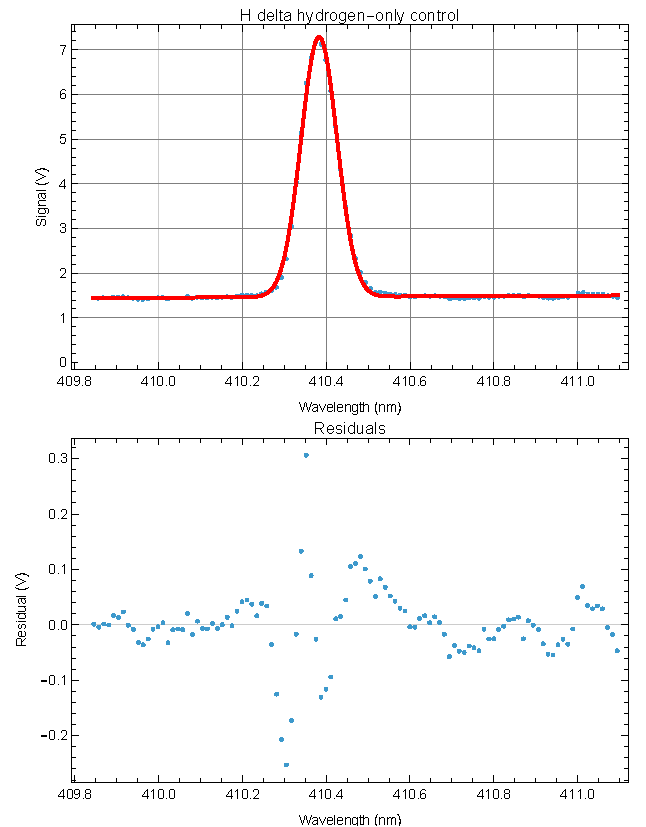
\includegraphics[width=0.48\textwidth]{PHASE1_real_wavelength_files/PHASE4_Hydrogen_only_control/fit_figures_no_tables/H_delta_hydrogen_only_fit_residual.pdf}
\caption{Hydrogen only control fits for H gamma and H delta.}
\end{figure}

\begin{figure}[H]
\centering
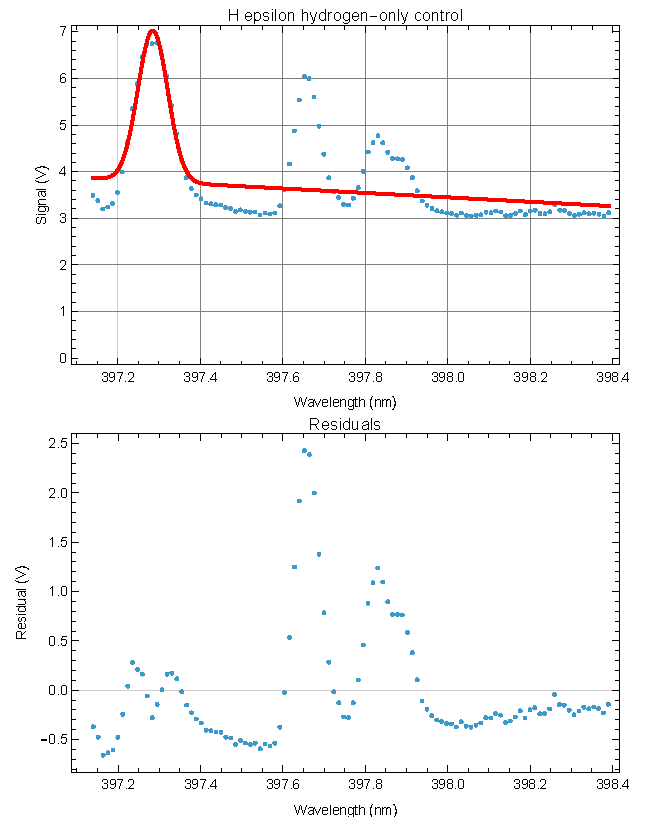
\includegraphics[width=0.48\textwidth]{PHASE1_real_wavelength_files/PHASE4_Hydrogen_only_control/fit_figures_no_tables/H_epsilon_hydrogen_only_fit_residual.pdf}
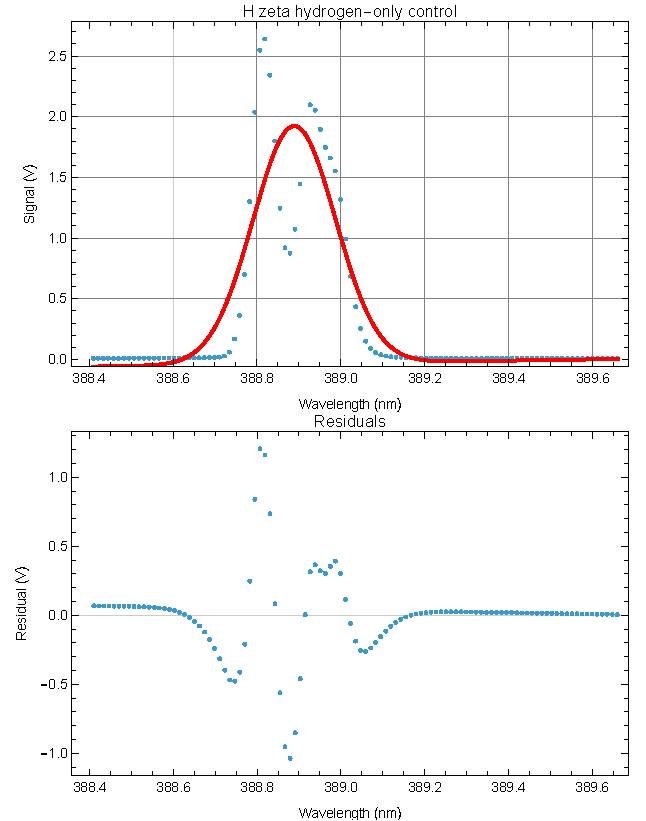
\includegraphics[width=0.48\textwidth]{PHASE1_real_wavelength_files/PHASE4_Hydrogen_only_control/fit_figures_no_tables/H_zeta_hydrogen_only_fit_residual.pdf}
\caption{Hydrogen only control fits for H epsilon and H zeta. These regions showed extra structure and were not used in the main fit.}
\end{figure}

\subsection{Line Checks}

The line identity maps were used to check the high order Balmer regions. They show that H epsilon and H zeta contain extra peaks that are also visible in the hydrogen only scans.

\begin{figure}[H]
\centering
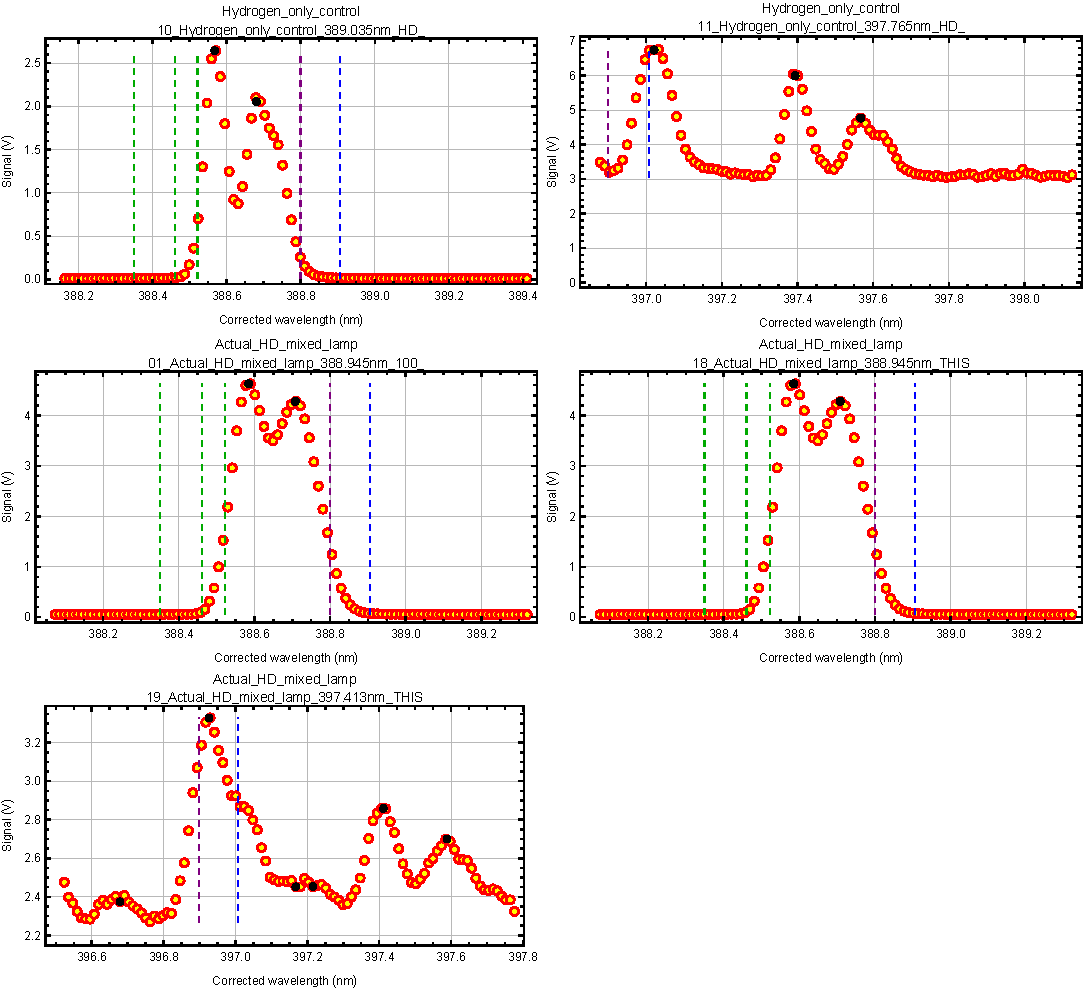
\includegraphics[width=0.95\textwidth]{PHASE1_real_wavelength_files/PHASE7_line_identity_map/figures/suspicious_regions_identity_summary.pdf}
\caption{Identity map summary for the suspicious H epsilon and H zeta regions. The zeta region overlaps possible first order oxygen aliases, and the epsilon region contains multiple extra peaks.}
\end{figure}

\subsection{Extra Models}

Two Gaussian checks were performed for H epsilon and H zeta because the single peak control fits showed extra structure. These checks were diagnostic and were not included in the main mass ratio fit.

\begin{figure}[H]
\centering
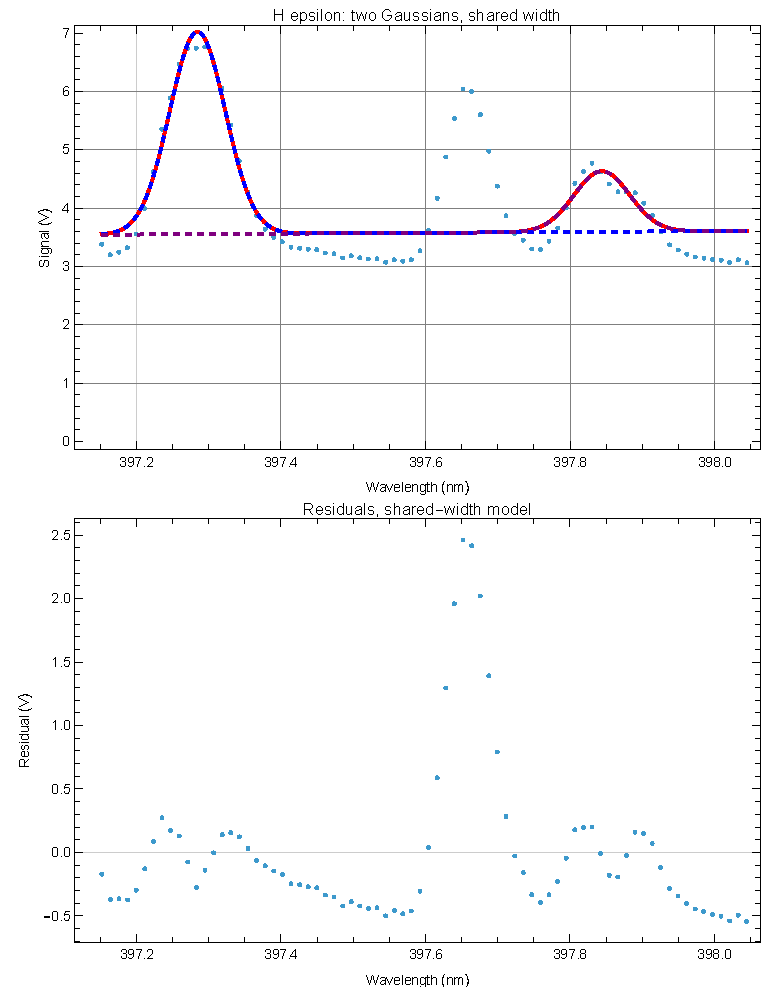
\includegraphics[width=0.48\textwidth]{PHASE1_real_wavelength_files/PHASE4_Hydrogen_only_two_gaussian_checks/fit_figures/H_epsilon_two_gaussian_shared_width.pdf}
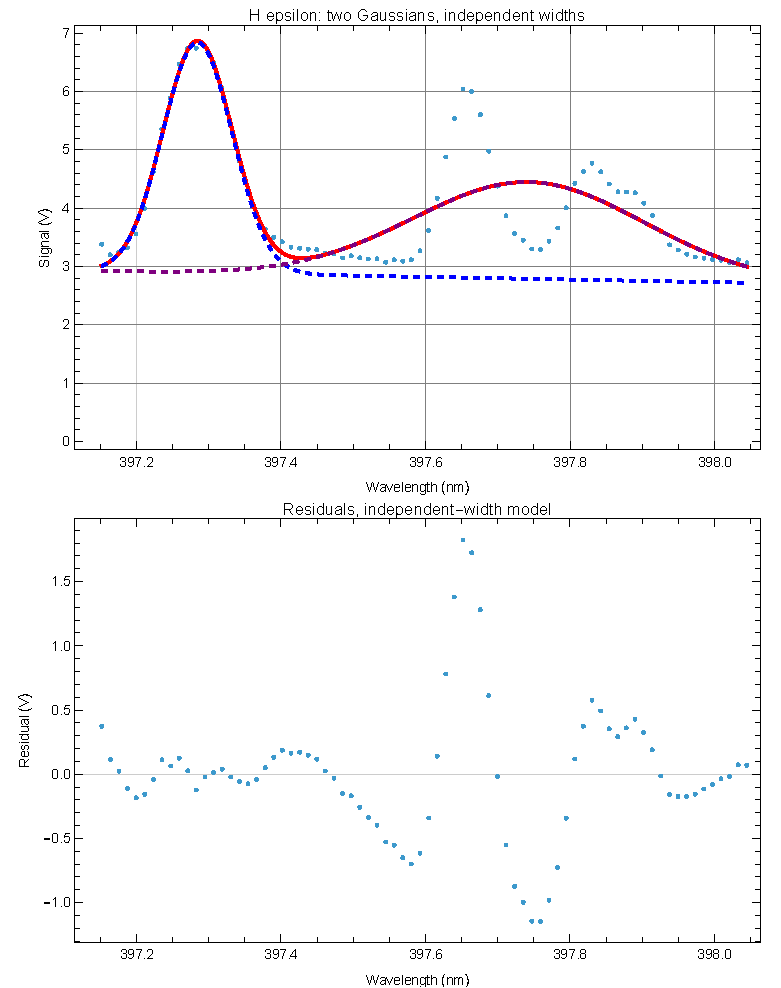
\includegraphics[width=0.48\textwidth]{PHASE1_real_wavelength_files/PHASE4_Hydrogen_only_two_gaussian_checks/fit_figures/H_epsilon_two_gaussian_independent_widths.pdf}
\caption{Two Gaussian diagnostic fits for H epsilon.}
\end{figure}

\begin{figure}[H]
\centering
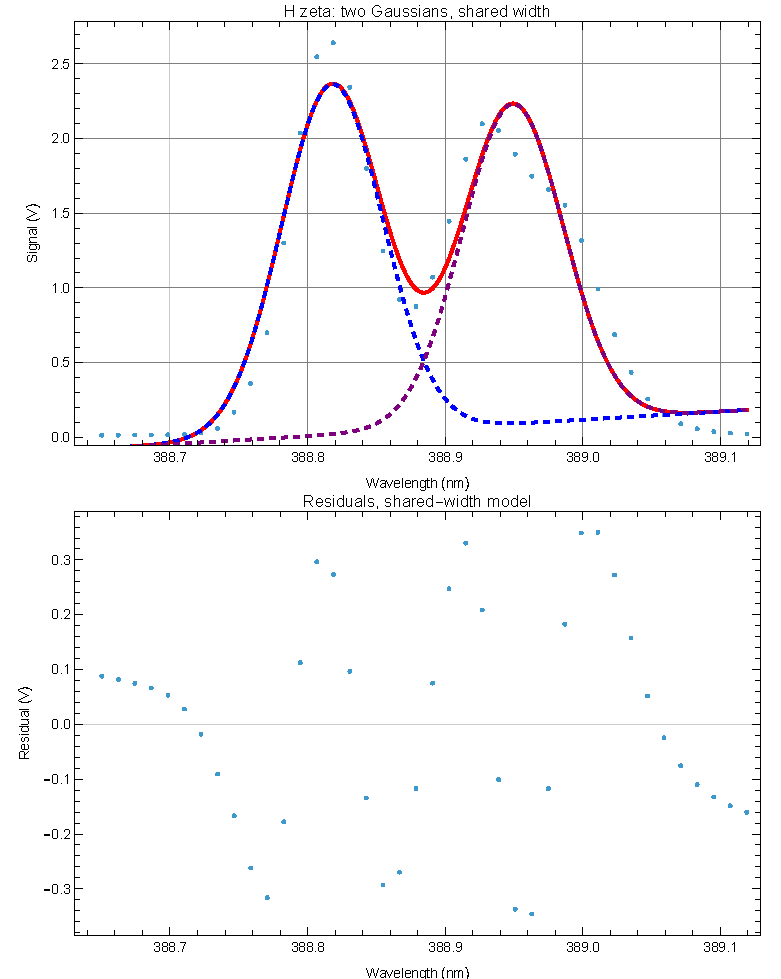
\includegraphics[width=0.48\textwidth]{PHASE1_real_wavelength_files/PHASE4_Hydrogen_only_two_gaussian_checks/fit_figures/H_zeta_two_gaussian_shared_width.pdf}
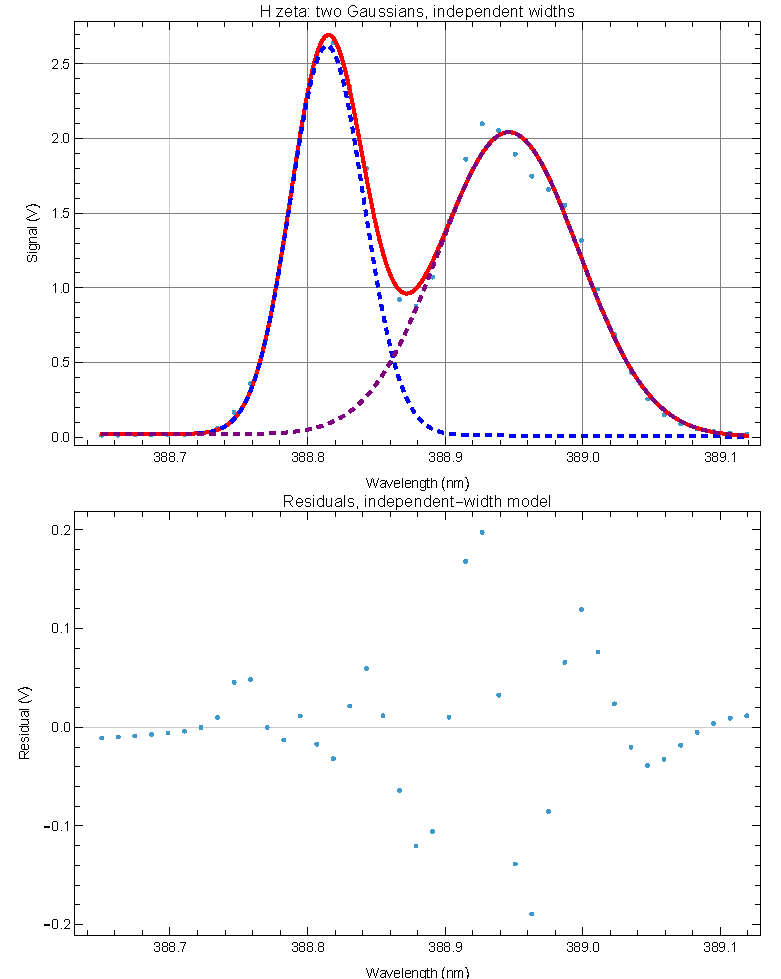
\includegraphics[width=0.48\textwidth]{PHASE1_real_wavelength_files/PHASE4_Hydrogen_only_two_gaussian_checks/fit_figures/H_zeta_two_gaussian_independent_widths.pdf}
\caption{Two Gaussian diagnostic fits for H zeta.}
\end{figure}

\begin{table}[H]
\centering
\caption{Two Gaussian diagnostic model comparison for H epsilon and H zeta.}
\resizebox{\textwidth}{!}{%
\begin{tabular}{llrrrrrrr}
\hline
Line & Model & \(\mu_H\) & \(\mu_I\) & \(\sigma_H\) & \(\sigma_I\) & RMS & AIC & BIC \\
\hline
H epsilon & one\_gaussian & 397.2841 &  & 0.0397 &  & 0.6788 & -48.90 & -37.24 \\
H epsilon & two\_gaussian\_shared\_width & 397.2846 & 397.8440 & 0.0386 & 0.0386 & 0.6348 & -55.08 & -38.76 \\
H epsilon & two\_gaussian\_independent\_widths & 397.2847 & 397.7428 & 0.0481 & 0.1594 & 0.5321 & -79.91 & -61.26 \\
H zeta & one\_gaussian & 388.8171 &  & 0.0240 &  & 0.6363 & -26.17 & -17.73 \\
H zeta & two\_gaussian\_shared\_width & 388.8180 & 388.9491 & 0.0368 & 0.0368 & 0.1987 & -115.27 & -103.45 \\
H zeta & two\_gaussian\_independent\_widths & 388.8143 & 388.9463 & 0.0266 & 0.0510 & 0.0707 & -195.99 & -182.48 \\%
\end{tabular}%
}
\end{table}

\subsection{Mixed Fits}

The first automatic mixed lamp fit was useful for diagnosing failures, but not all of its outputs were used. The final analysis used a global constrained fit, but the intermediate fits are included here for transparency.

\begin{figure}[H]
\centering
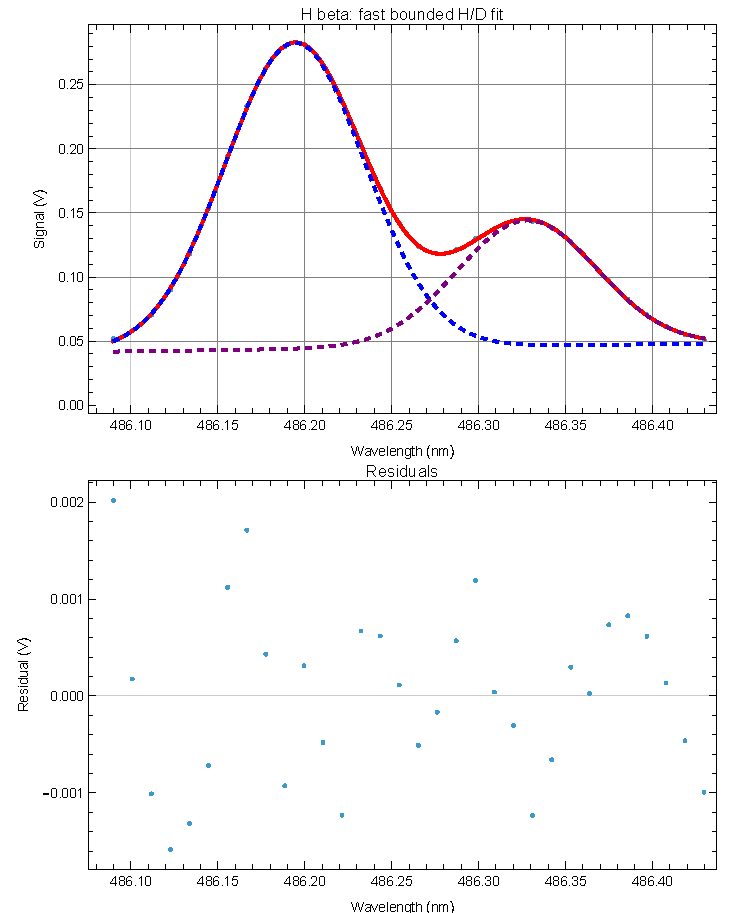
\includegraphics[width=0.48\textwidth]{PHASE1_real_wavelength_files/PHASE5C_actual_HD_fast_bounded_refit/fit_figures_no_tables/H_beta_fast_bounded_HD_fit.pdf}
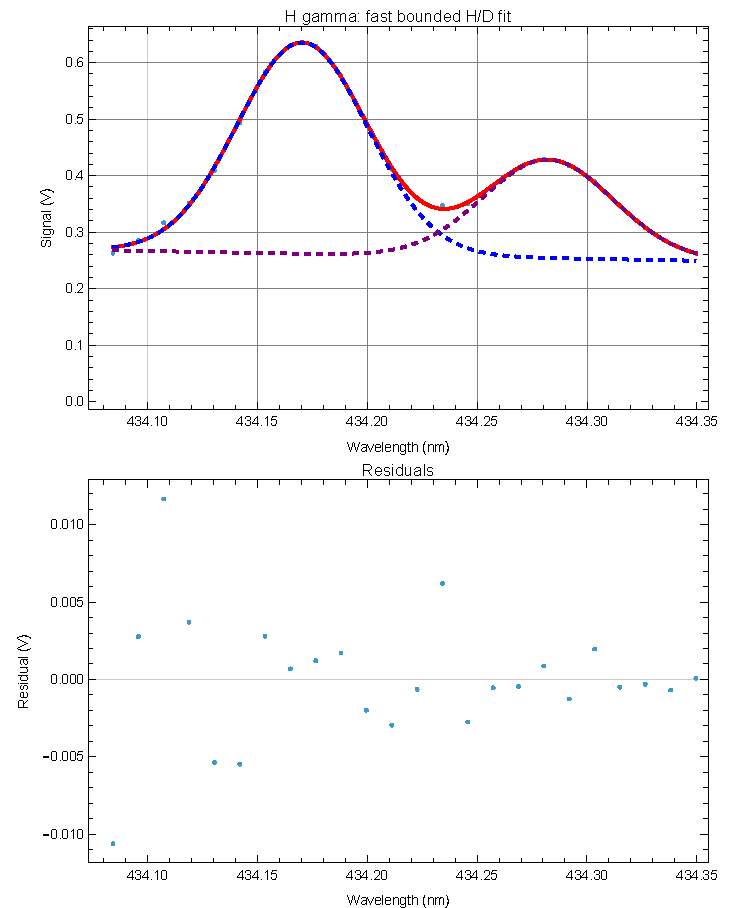
\includegraphics[width=0.48\textwidth]{PHASE1_real_wavelength_files/PHASE5C_actual_HD_fast_bounded_refit/fit_figures_no_tables/H_gamma_fast_bounded_HD_fit.pdf}
\caption{Fast bounded hydrogen deuterium fits for H beta and H gamma.}
\end{figure}

\begin{figure}[H]
\centering
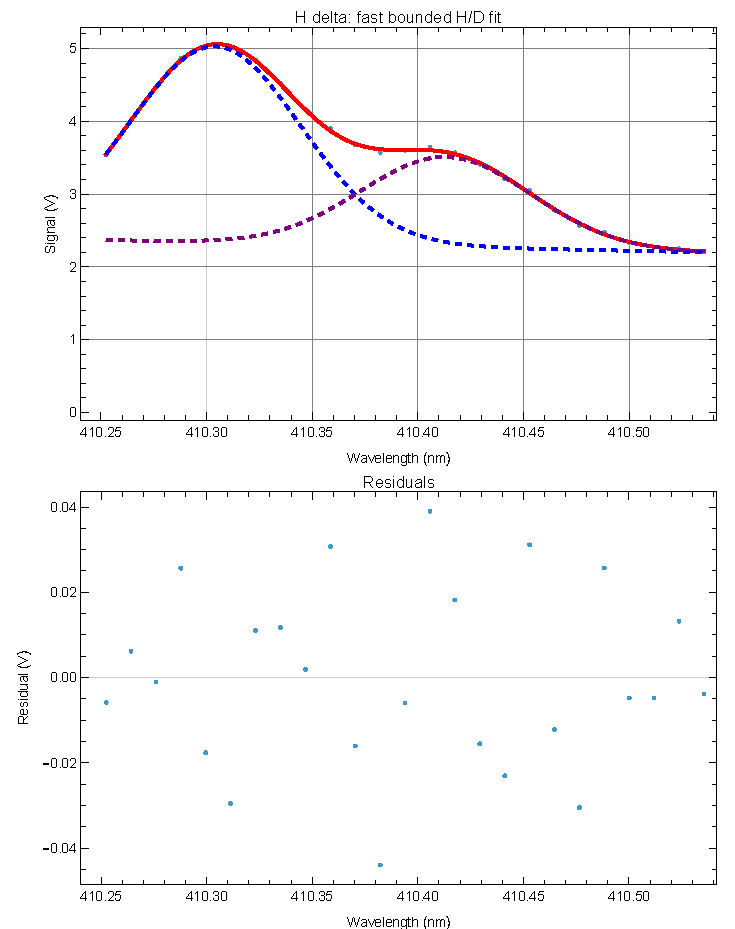
\includegraphics[width=0.48\textwidth]{PHASE1_real_wavelength_files/PHASE5C_actual_HD_fast_bounded_refit/fit_figures_no_tables/H_delta_fast_bounded_HD_fit.pdf}
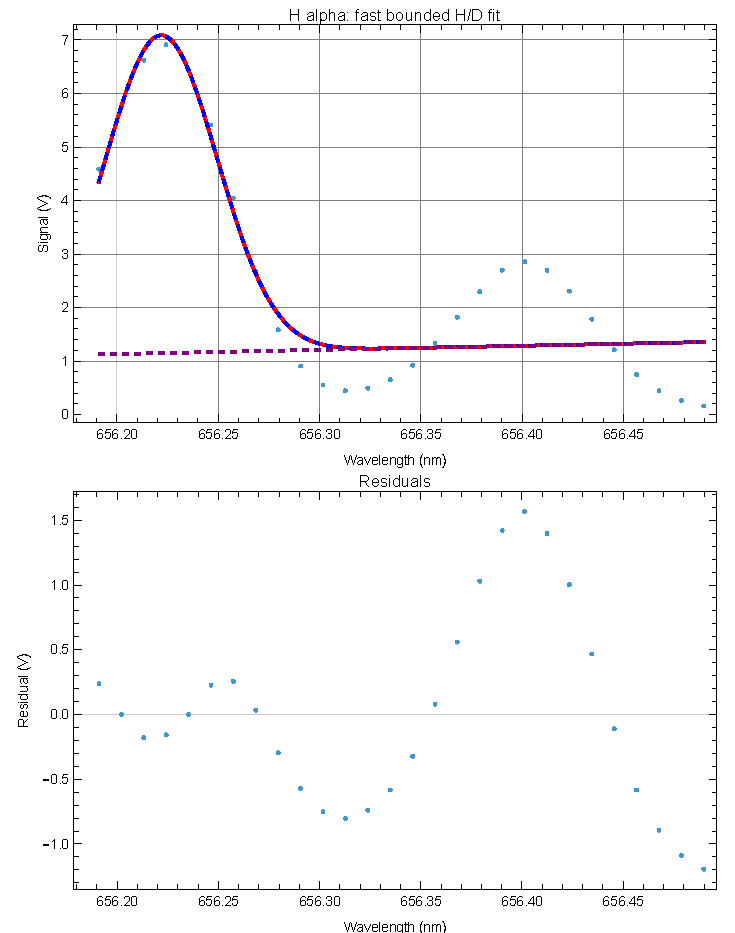
\includegraphics[width=0.48\textwidth]{PHASE1_real_wavelength_files/PHASE5C_actual_HD_fast_bounded_refit/fit_figures_no_tables/H_alpha_fast_bounded_HD_fit.pdf}
\caption{Fast bounded fits for H delta and H alpha. The H alpha fit is shown here to document why a local refit was used instead.}
\end{figure}

\begin{figure}[H]
\centering
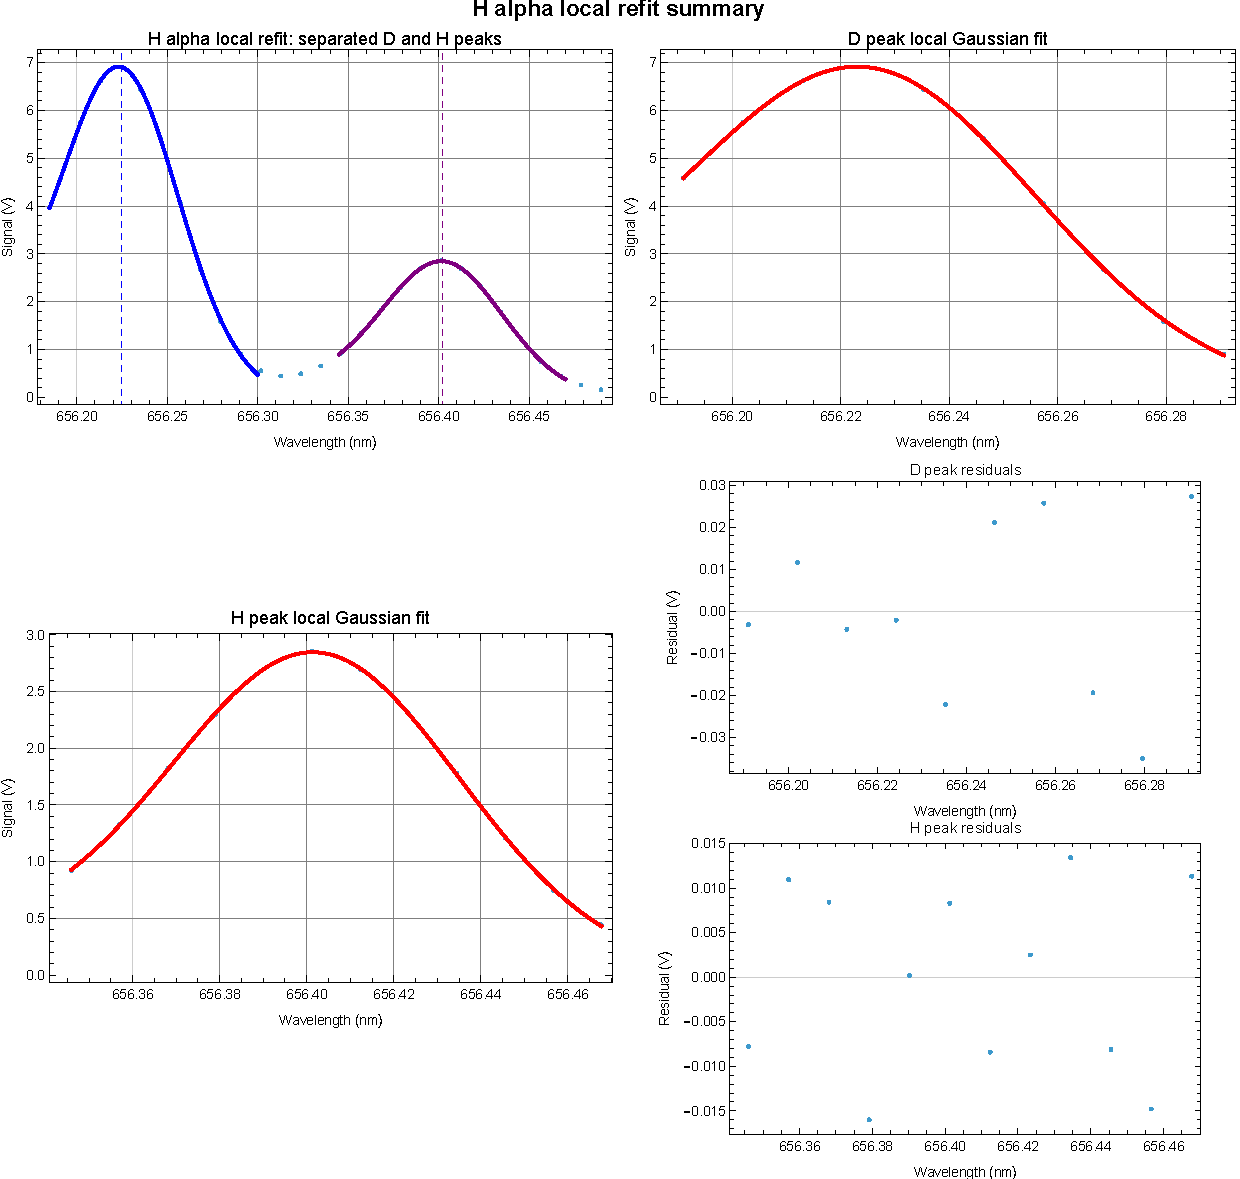
\includegraphics[width=0.95\textwidth]{PHASE1_real_wavelength_files/PHASE5D_H_alpha_local_refit/H_alpha_local_refit_2x2_collage.pdf}
\caption{Compact local H alpha refit summary.}
\end{figure}

\begin{table}[H]
\centering
\caption{Fast bounded hydrogen deuterium fit table. H alpha was replaced by the local refit in the separate peak analysis.}
\begin{tabular}{lrrrrrrr}
\hline
Line & \(\mu_D\) & \(\mu_H\) & \(\Delta\lambda\) & \(\lambda_H\) & \(\Delta\lambda_c\) & Error & RMS \\
\hline
H alpha & 656.2218 & 656.4518 & 0.23000 & 655.7422 & 0.22960 & 0.00038 & 0.7475 \\
H beta & 486.1944 & 486.3279 & 0.13352 & 485.9119 & 0.13329 & 0.00037 & 0.0009 \\
H gamma & 434.1705 & 434.2823 & 0.11174 & 433.9561 & 0.11155 & 0.00070 & 0.0041 \\
H delta & 410.3041 & 410.4134 & 0.10928 & 410.1284 & 0.10909 & 0.00099 & 0.0209 \\%
\end{tabular}
\end{table}

\begin{table}[H]
\centering
\caption{Local H alpha refit table.}
\begin{tabular}{lrrrrrr}
\hline
Line & \(\mu_D\) & \(\mu_H\) & \(\Delta\lambda\) & \(\lambda_H\) & \(\Delta\lambda_c\) & Error \\
\hline
H alpha & 656.2247 & 656.4022 & 0.17756 & 655.6927 & 0.17726 & 0.00066 \\
\end{tabular}
\end{table}

\subsection{Response Model}

The empirical response model used the measured Hg 546 nm line shape as a peak template. This was a check on the Gaussian line shape assumption.

\begin{figure}[H]
\centering
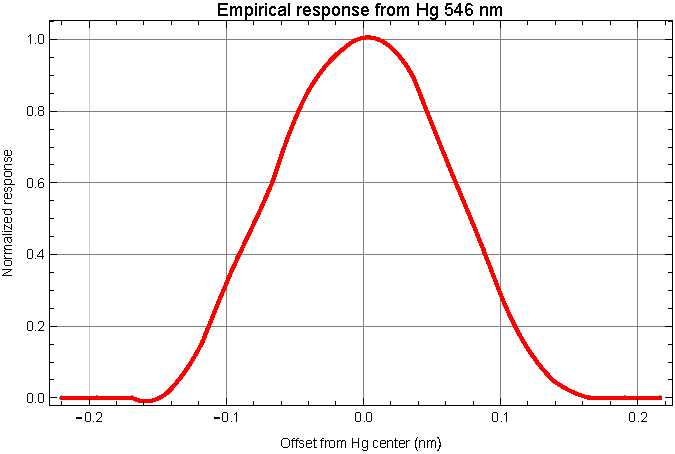
\includegraphics[width=0.42\textwidth]{PHASE1_real_wavelength_files/PHASE8_empirical_response_model/figures/empirical_Hg_546_response_template.pdf}
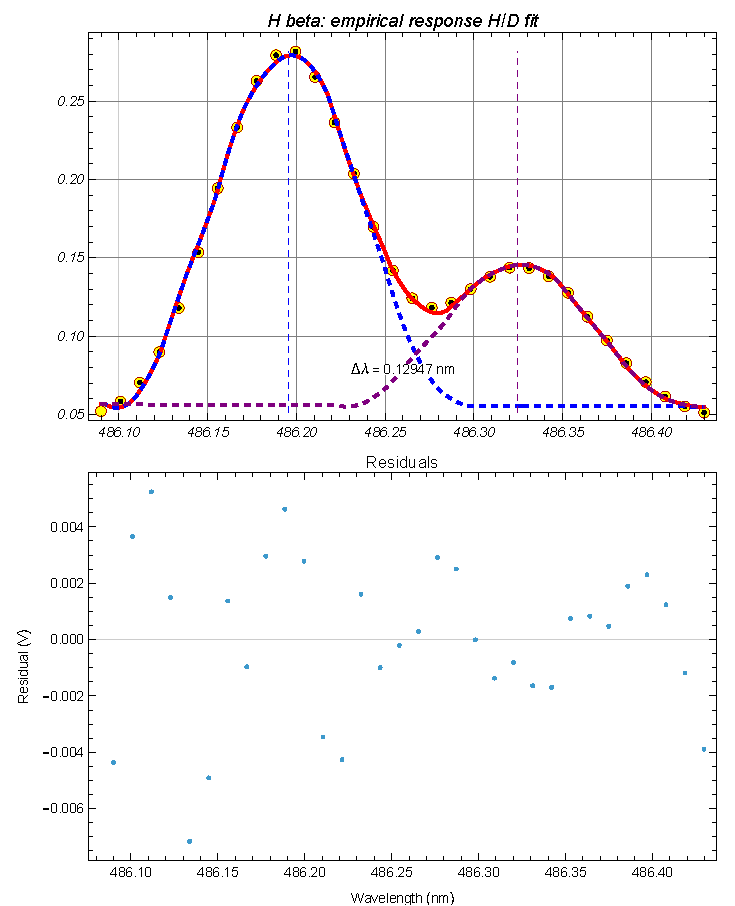
\includegraphics[width=0.48\textwidth]{PHASE1_real_wavelength_files/PHASE8_empirical_response_model/figures/H_beta_empirical_response_fit.pdf}
\caption{Empirical response model. Left: response template measured from Hg 546 nm. Right: empirical response fit for H beta.}
\end{figure}

\begin{figure}[H]
\centering
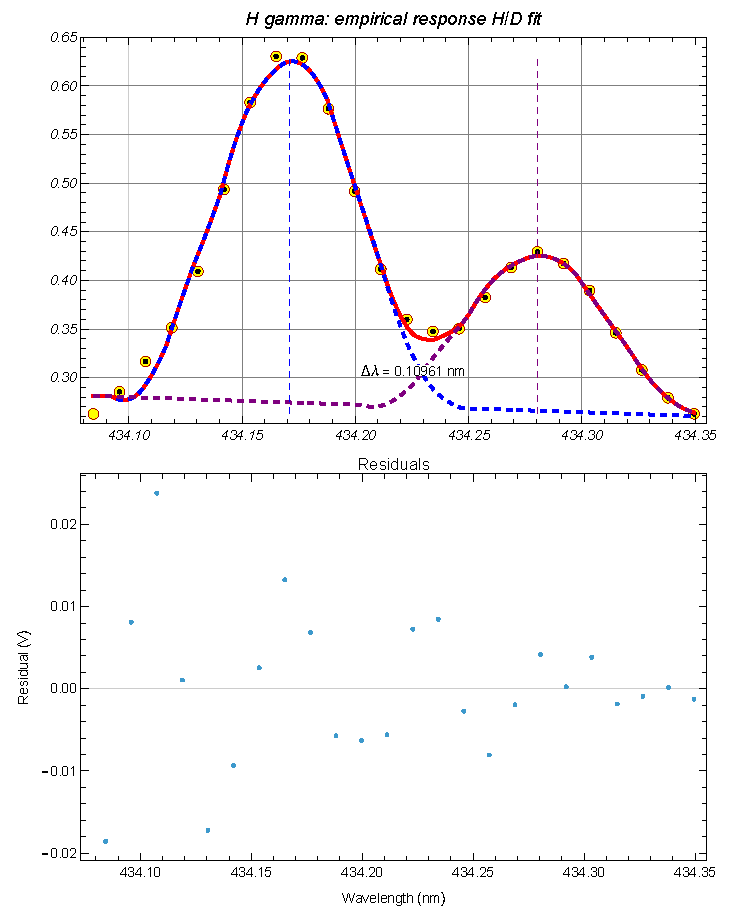
\includegraphics[width=0.48\textwidth]{PHASE1_real_wavelength_files/PHASE8_empirical_response_model/figures/H_gamma_empirical_response_fit.pdf}
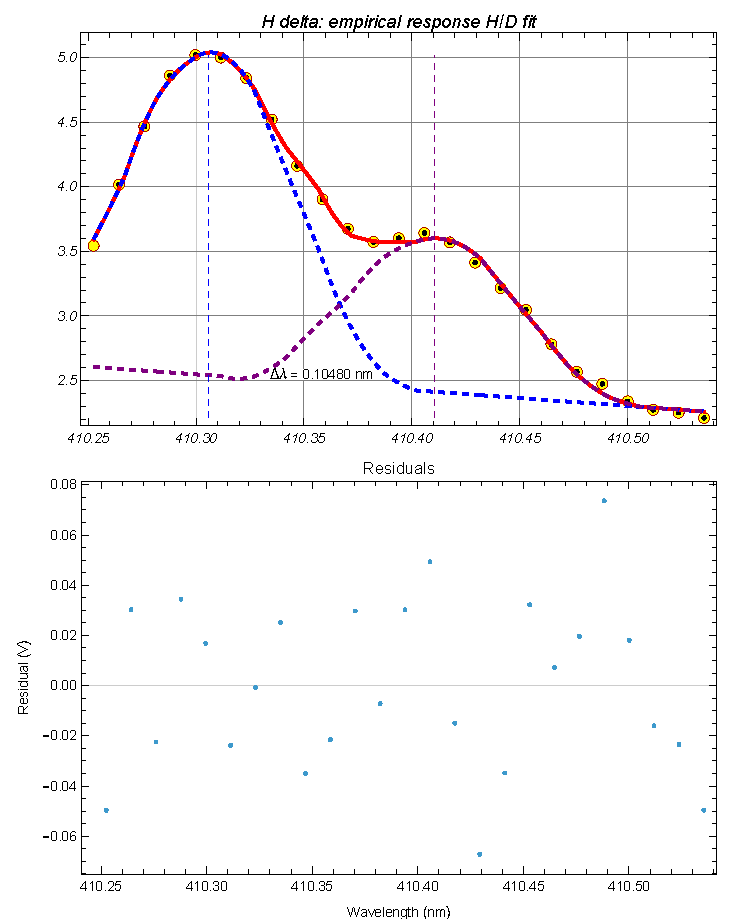
\includegraphics[width=0.48\textwidth]{PHASE1_real_wavelength_files/PHASE8_empirical_response_model/figures/H_delta_empirical_response_fit.pdf}
\caption{Empirical response fits for H gamma and H delta.}
\end{figure}

\begin{figure}[H]
\centering
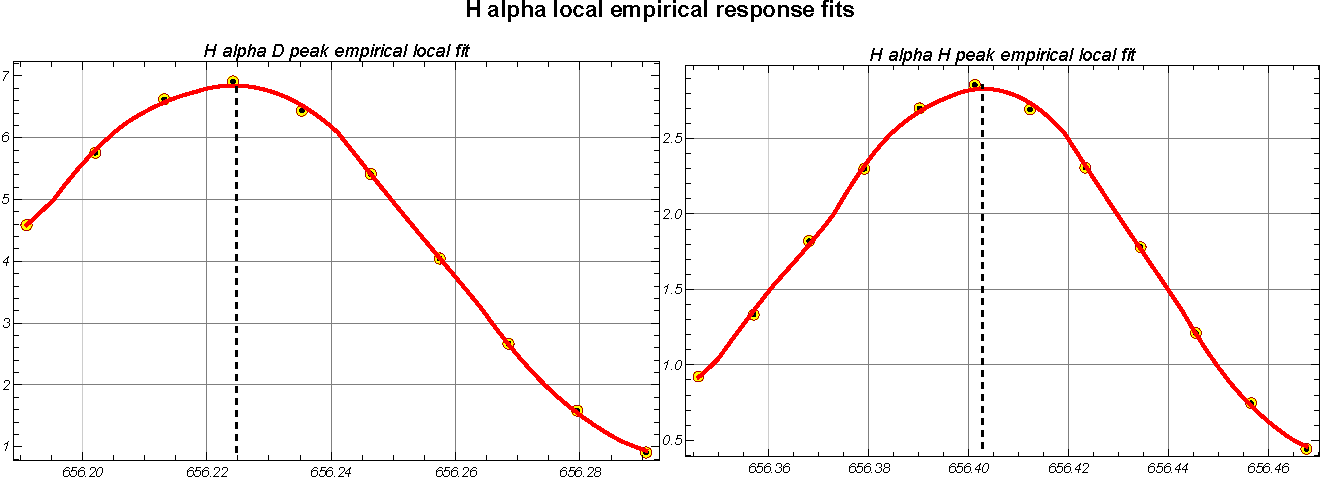
\includegraphics[width=0.48\textwidth]{PHASE1_real_wavelength_files/PHASE8B_empirical_alpha_local_and_exclusion/figures/H_alpha_local_empirical_response_fits.pdf}
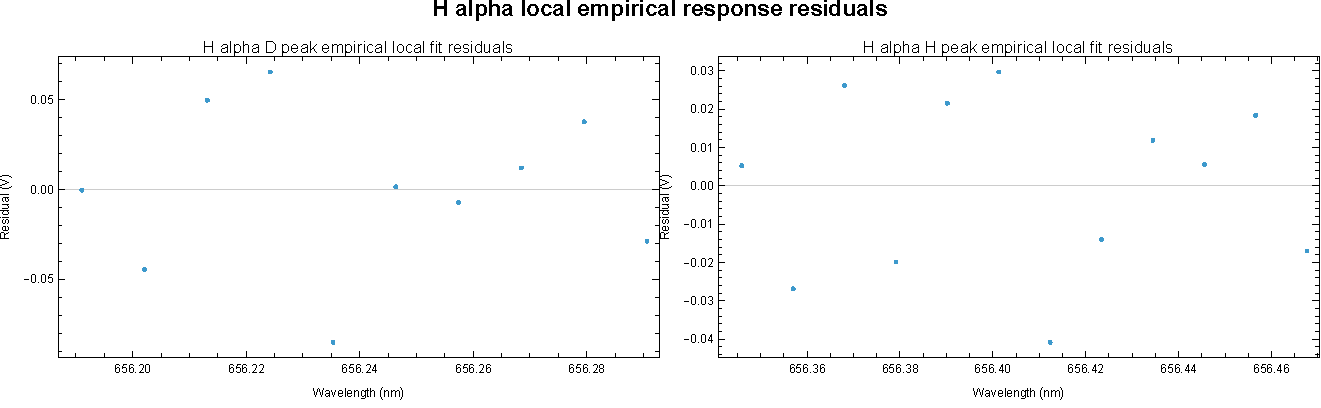
\includegraphics[width=0.48\textwidth]{PHASE1_real_wavelength_files/PHASE8B_empirical_alpha_local_and_exclusion/figures/H_alpha_local_empirical_response_residuals.pdf}
\caption{Local empirical response fits for H alpha. This was used to check whether the empirical response model could recover a reasonable H alpha separation when fit locally.}
\end{figure}

\subsection{Global Fits}

These figures show the spectra used in the global physics constrained fit. The fit shares one isotope shift slope across all four usable Balmer lines.

\begin{figure}[H]
\centering
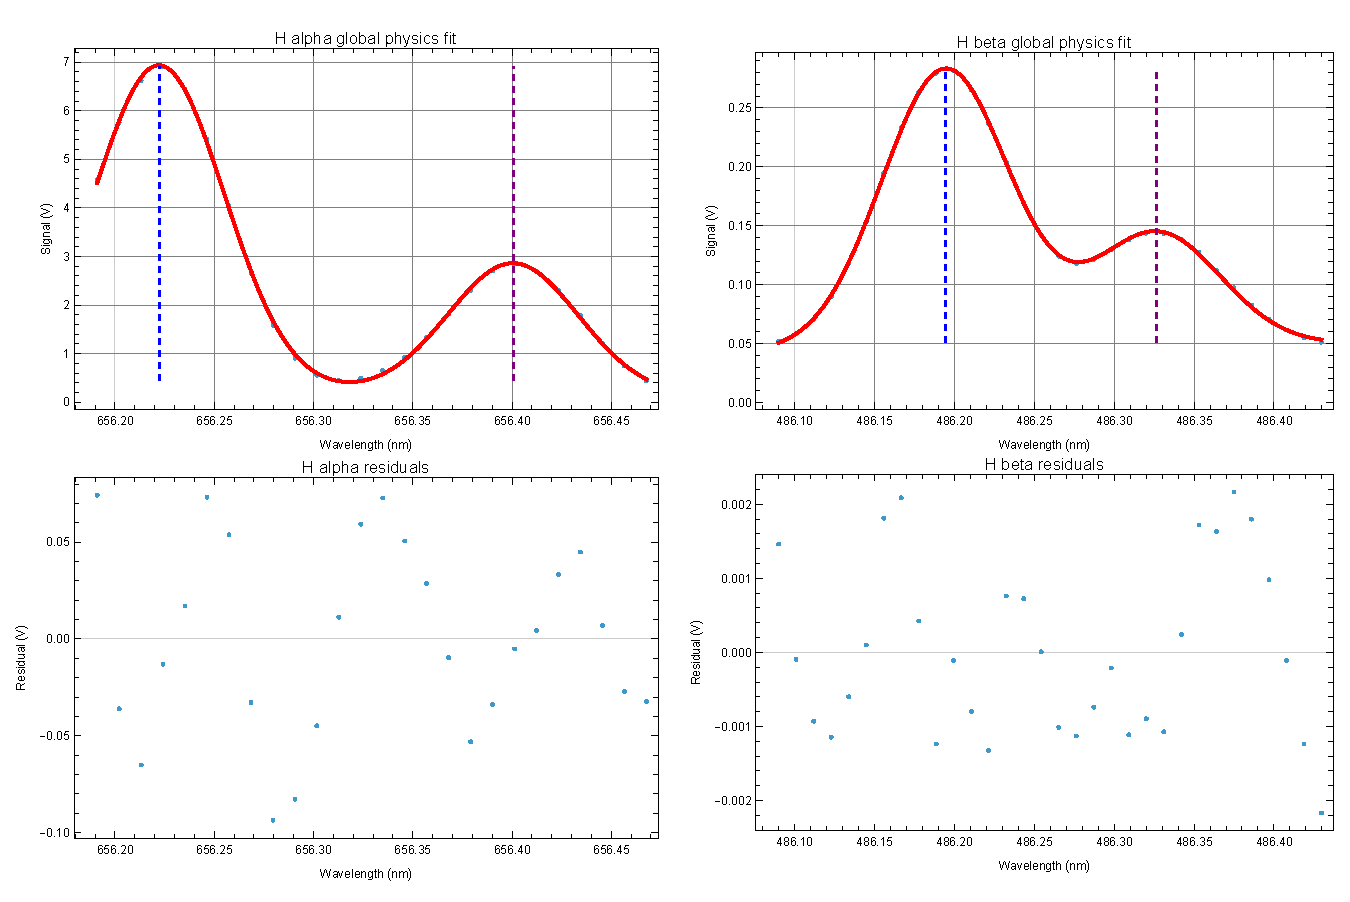
\includegraphics[width=0.95\textwidth]{PHASE1_real_wavelength_files/PHASE10_global_physics_constrained_fit/figures/global_physics_fit_alpha_beta.pdf}
\caption{Global physics constrained fit for H alpha and H beta.}
\end{figure}

\begin{figure}[H]
\centering
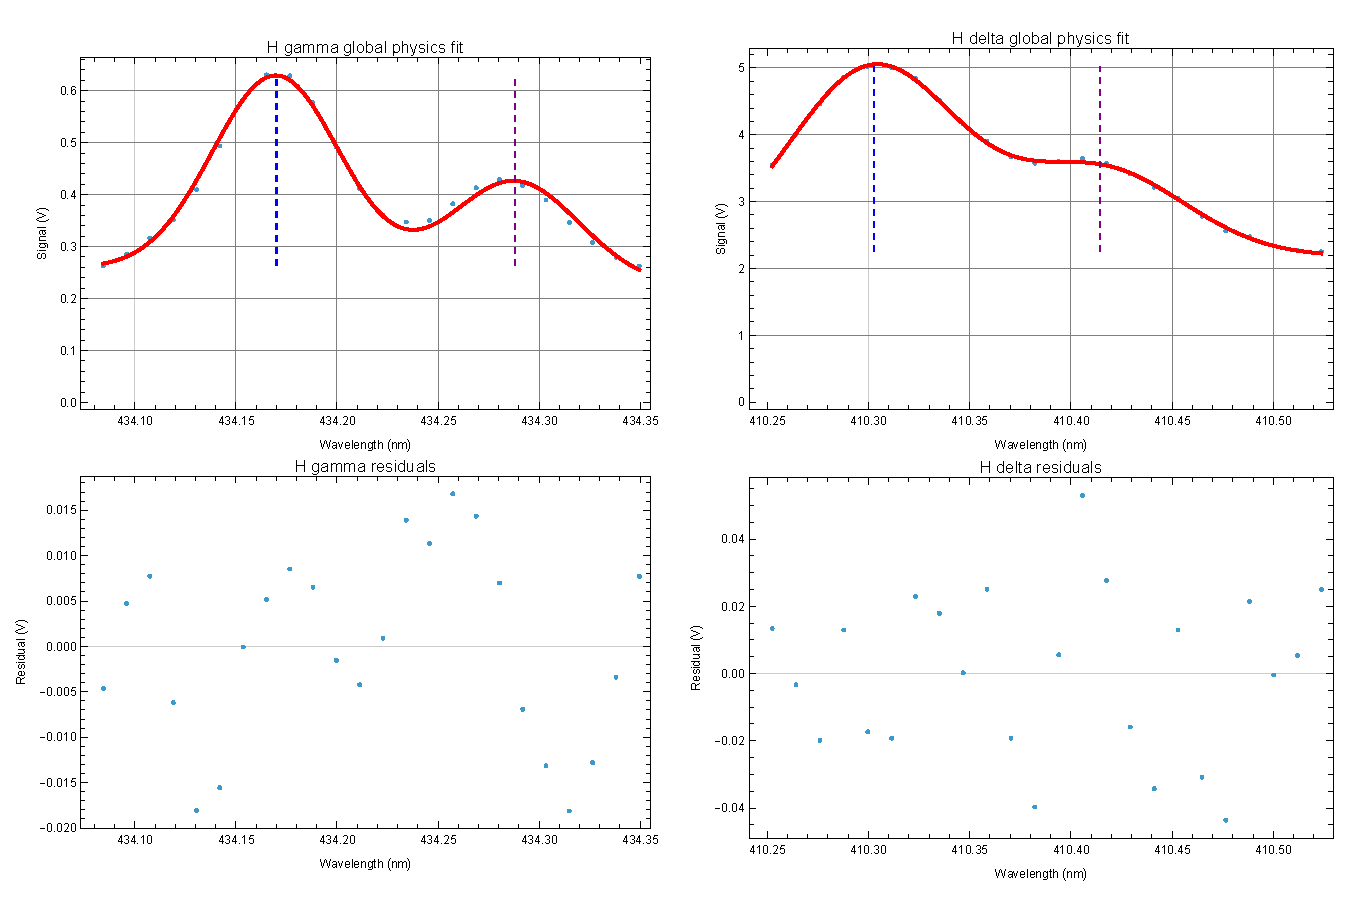
\includegraphics[width=0.95\textwidth]{PHASE1_real_wavelength_files/PHASE10_global_physics_constrained_fit/figures/global_physics_fit_gamma_delta.pdf}
\caption{Global physics constrained fit for H gamma and H delta.}
\end{figure}

\subsection{Fit Checks}

The first automatic hydrogen deuterium fits are shown here as diagnostic checks. These figures are not all used in the final physics result, but they document why the analysis moved to bounded fits and a local H alpha refit.

\begin{figure}[H]
\centering
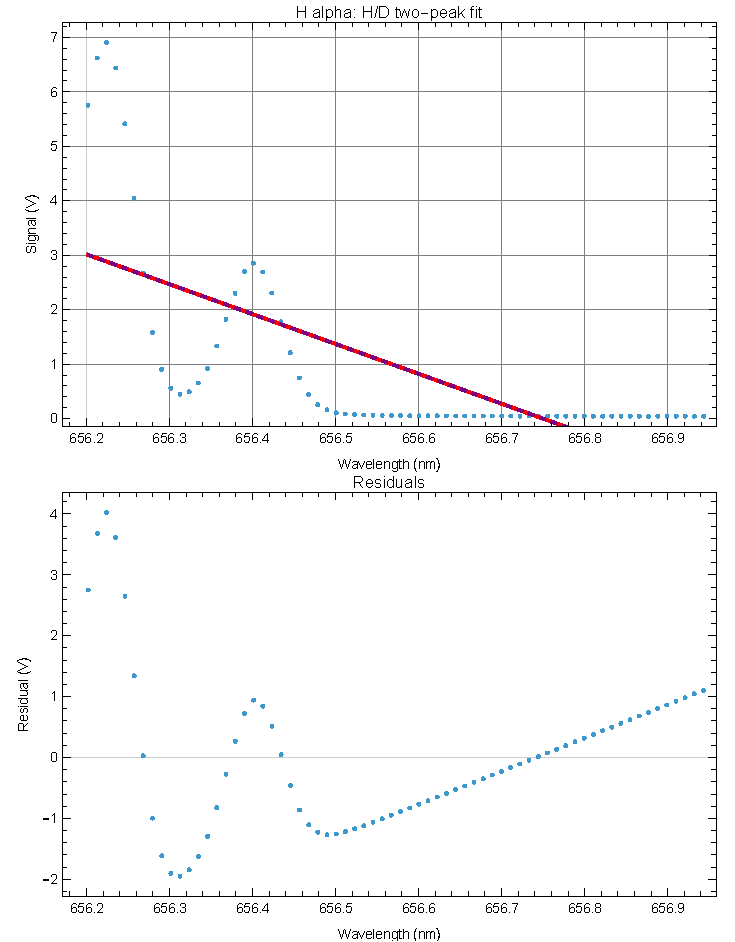
\includegraphics[width=0.48\textwidth]{PHASE1_real_wavelength_files/PHASE5_actual_HD_two_peak_fits/fit_figures_no_tables/H_alpha_actual_HD_two_peak_fit.pdf}
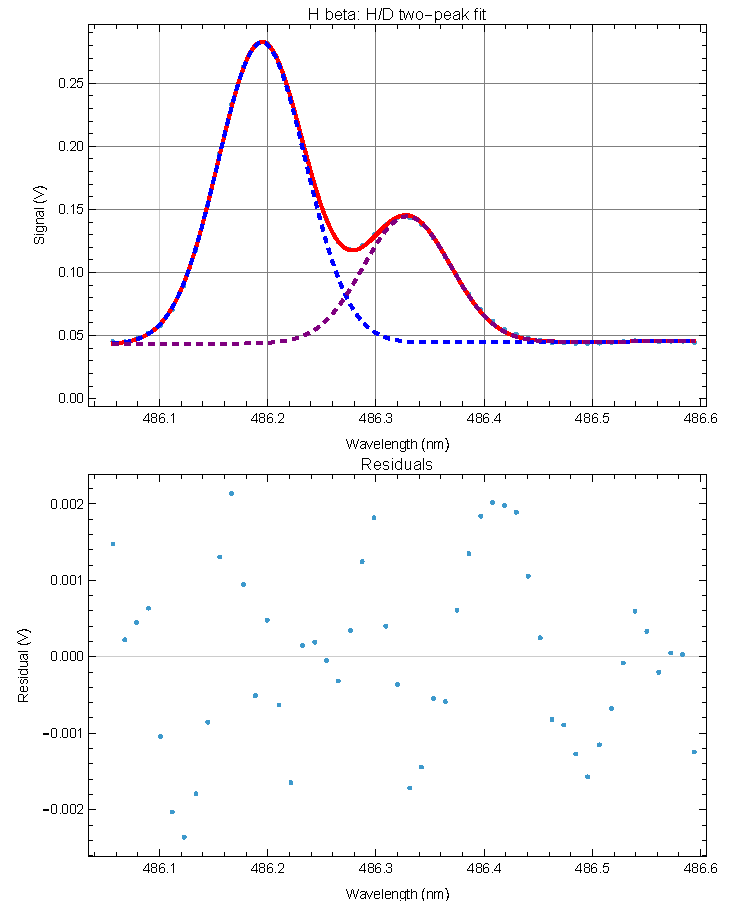
\includegraphics[width=0.48\textwidth]{PHASE1_real_wavelength_files/PHASE5_actual_HD_two_peak_fits/fit_figures_no_tables/H_beta_actual_HD_two_peak_fit.pdf}
\caption{Initial automatic mixed lamp fits for H alpha and H beta.}
\end{figure}

\begin{figure}[H]
\centering
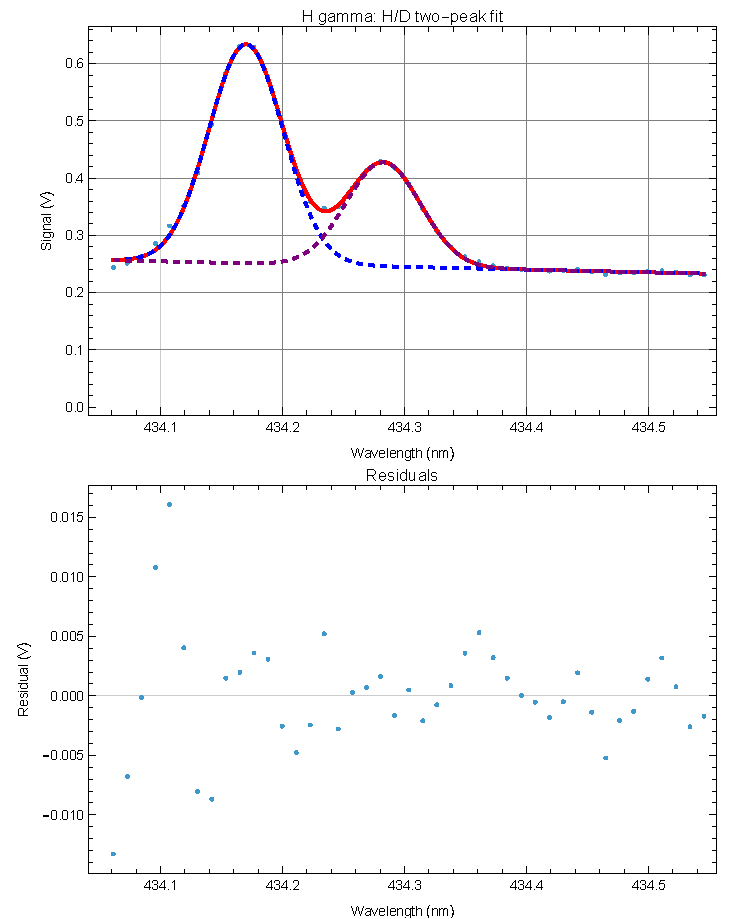
\includegraphics[width=0.48\textwidth]{PHASE1_real_wavelength_files/PHASE5_actual_HD_two_peak_fits/fit_figures_no_tables/H_gamma_actual_HD_two_peak_fit.pdf}
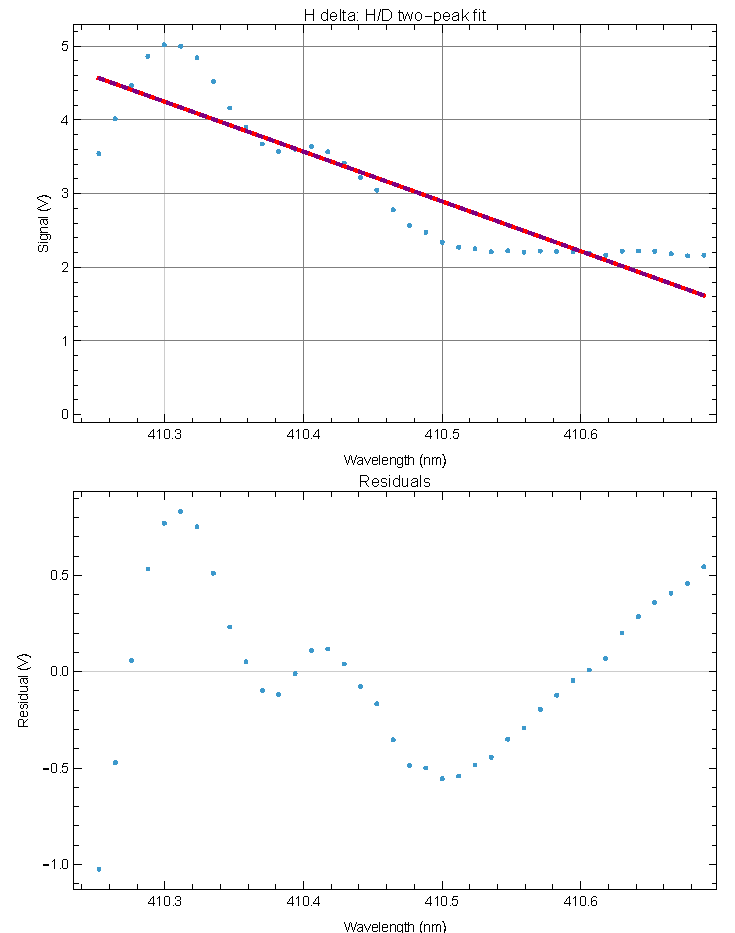
\includegraphics[width=0.48\textwidth]{PHASE1_real_wavelength_files/PHASE5_actual_HD_two_peak_fits/fit_figures_no_tables/H_delta_actual_HD_two_peak_fit.pdf}
\caption{Initial automatic mixed lamp fits for H gamma and H delta.}
\end{figure}

\begin{figure}[H]
\centering
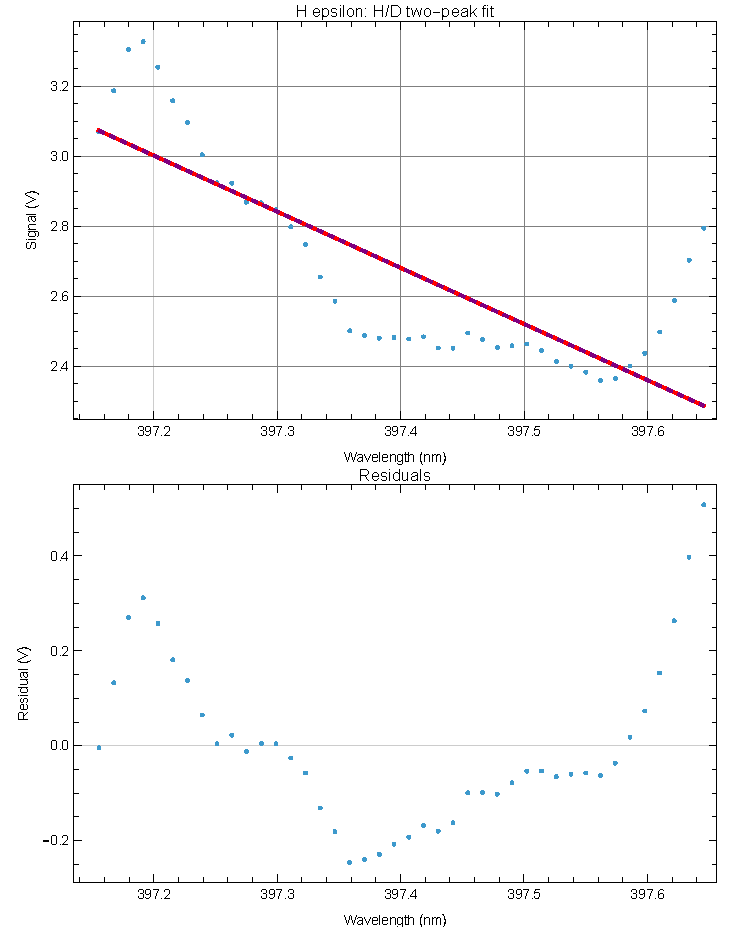
\includegraphics[width=0.48\textwidth]{PHASE1_real_wavelength_files/PHASE5_actual_HD_two_peak_fits/fit_figures_no_tables/H_epsilon_actual_HD_two_peak_fit.pdf}
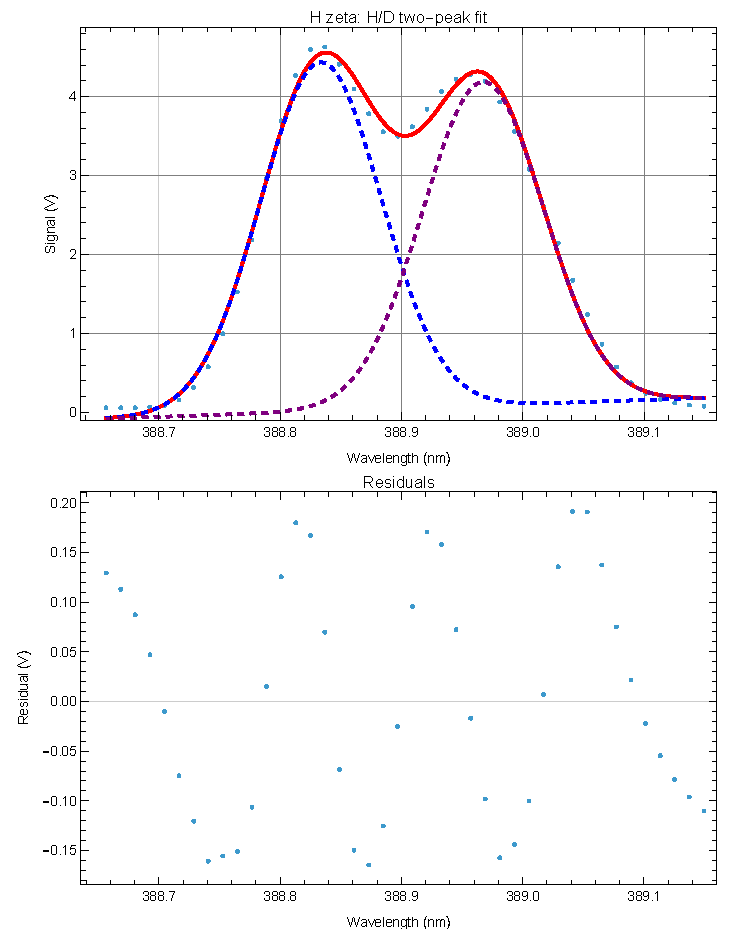
\includegraphics[width=0.48\textwidth]{PHASE1_real_wavelength_files/PHASE5_actual_HD_two_peak_fits/fit_figures_no_tables/H_zeta_actual_HD_two_peak_fit.pdf}
\caption{Initial automatic mixed lamp fits for H epsilon and H zeta. These were treated as diagnostics only.}
\end{figure}

\subsection{CurveFit Checks}

CurveFit reports were kept in the final PDF as appendix material because CurveFit was part of the lab workflow. The final numerical results still come from the Mathematica fits in the main analysis.

\begin{figure}[H]
\centering
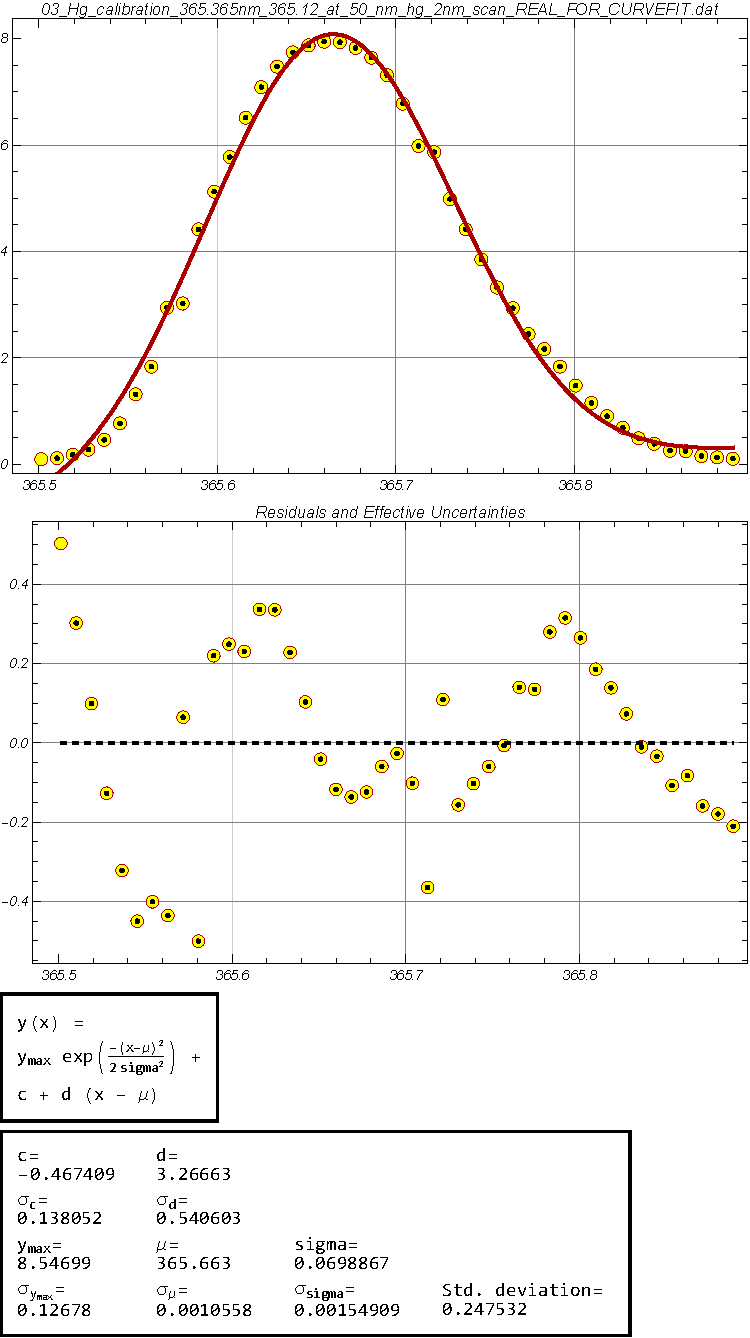
\includegraphics[width=\textwidth,height=0.78\textheight,keepaspectratio]{CurveFit_appendix/Hg_calibration_fit_reports/CF_Hg_365p119_GaussianLFit_appendix.pdf}
\caption{CurveFit Gaussian plus linear fit, 365.119 nm Hg line.}
\end{figure}

\begin{figure}[H]
\centering
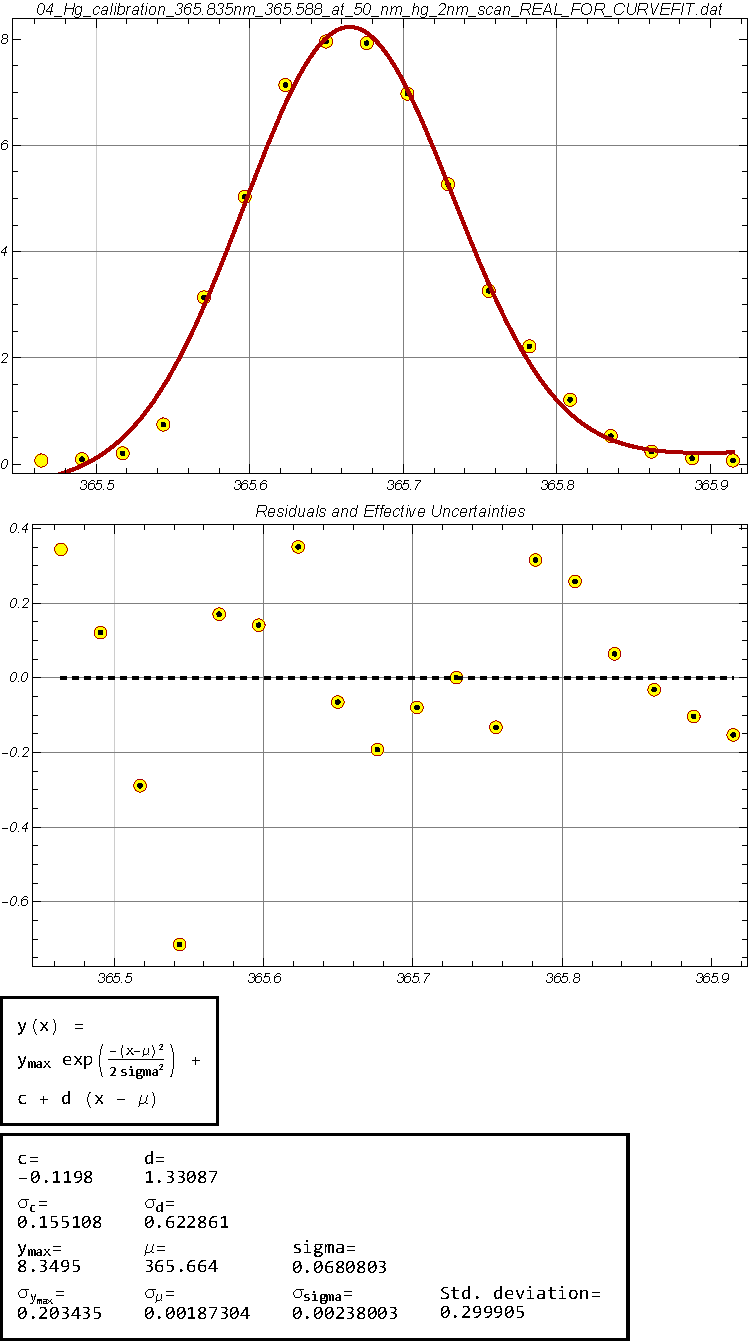
\includegraphics[width=\textwidth,height=0.78\textheight,keepaspectratio]{CurveFit_appendix/Hg_calibration_fit_reports/CF_Hg_365p588_GaussianLFit_appendix.pdf}
\caption{CurveFit Gaussian plus linear fit, 365.588 nm Hg line.}
\end{figure}

\begin{figure}[H]
\centering
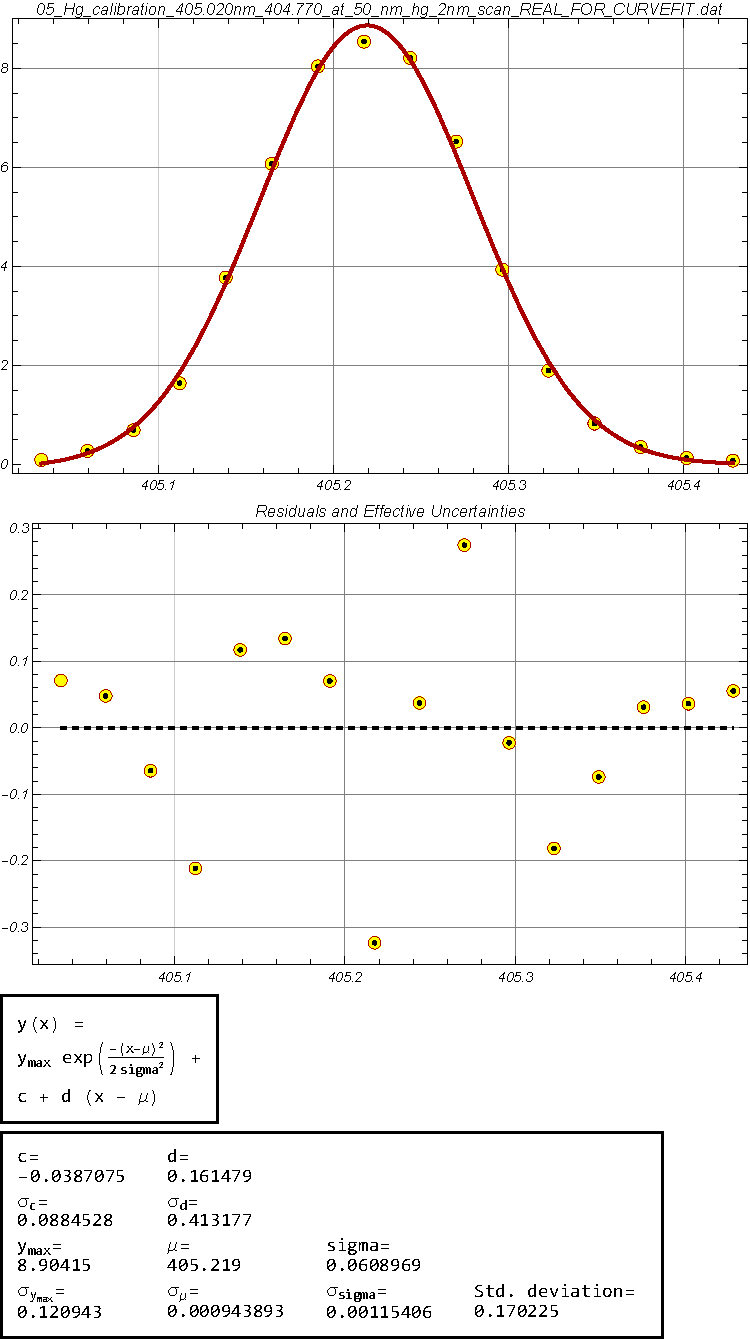
\includegraphics[width=\textwidth,height=0.78\textheight,keepaspectratio]{CurveFit_appendix/Hg_calibration_fit_reports/CF_Hg_404p770_GaussianLFit_appendix.pdf}
\caption{CurveFit Gaussian plus linear fit, 404.770 nm Hg line.}
\end{figure}

\begin{figure}[H]
\centering
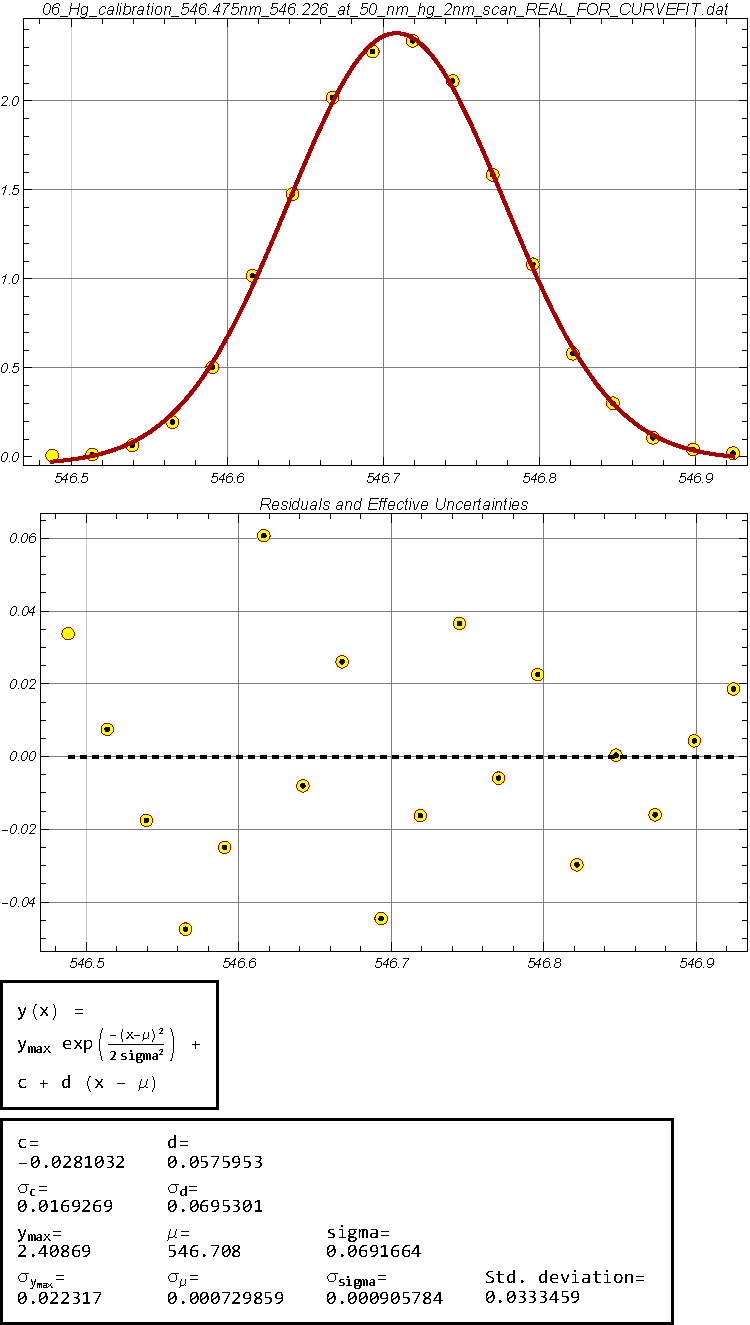
\includegraphics[width=\textwidth,height=0.78\textheight,keepaspectratio]{CurveFit_appendix/Hg_calibration_fit_reports/CF_Hg_546p226_GaussianLFit_appendix.pdf}
\caption{CurveFit Gaussian plus linear fit, 546.226 nm Hg line.}
\end{figure}

\begin{figure}[H]
\centering
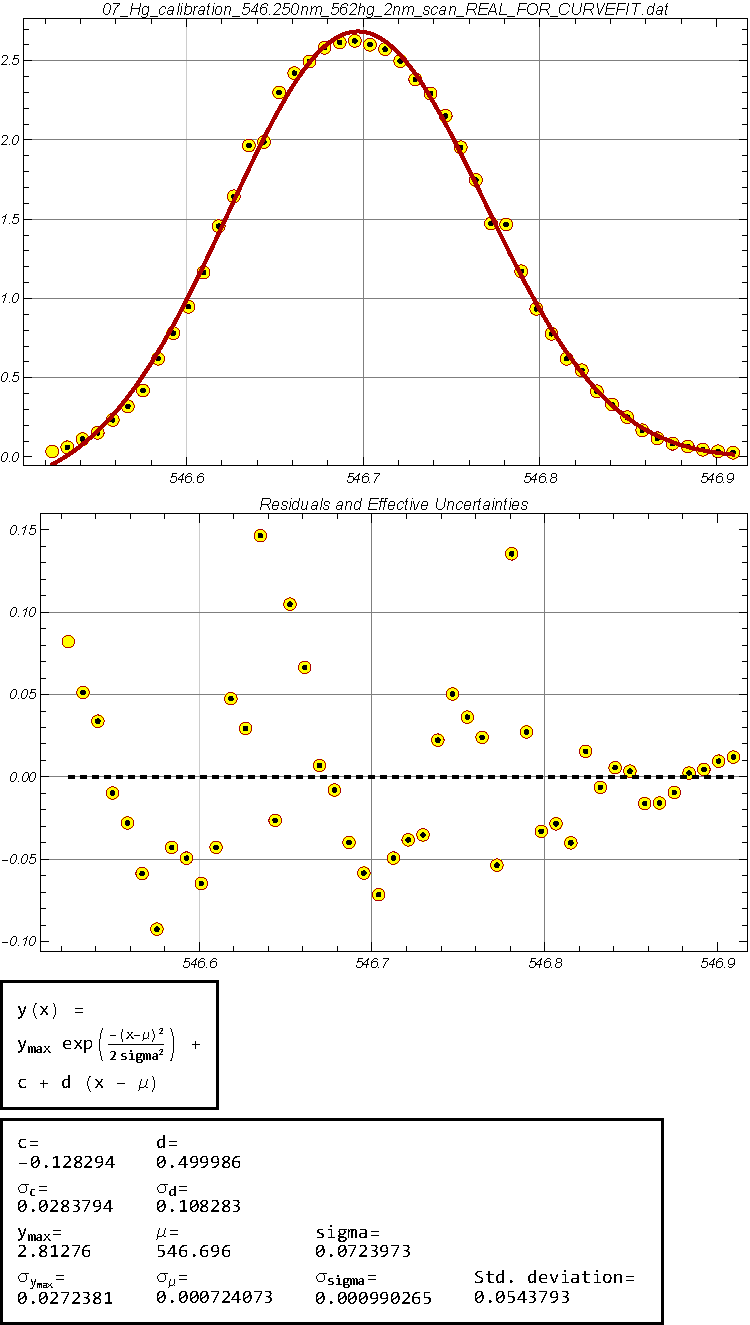
\includegraphics[width=\textwidth,height=0.78\textheight,keepaspectratio]{CurveFit_appendix/Hg_calibration_fit_reports/CF_Hg_546_repeat_wide_scan_appendix.pdf}
\caption{CurveFit repeat scan at 546 nm, wide slit configuration.}
\end{figure}

\begin{figure}[H]
\centering
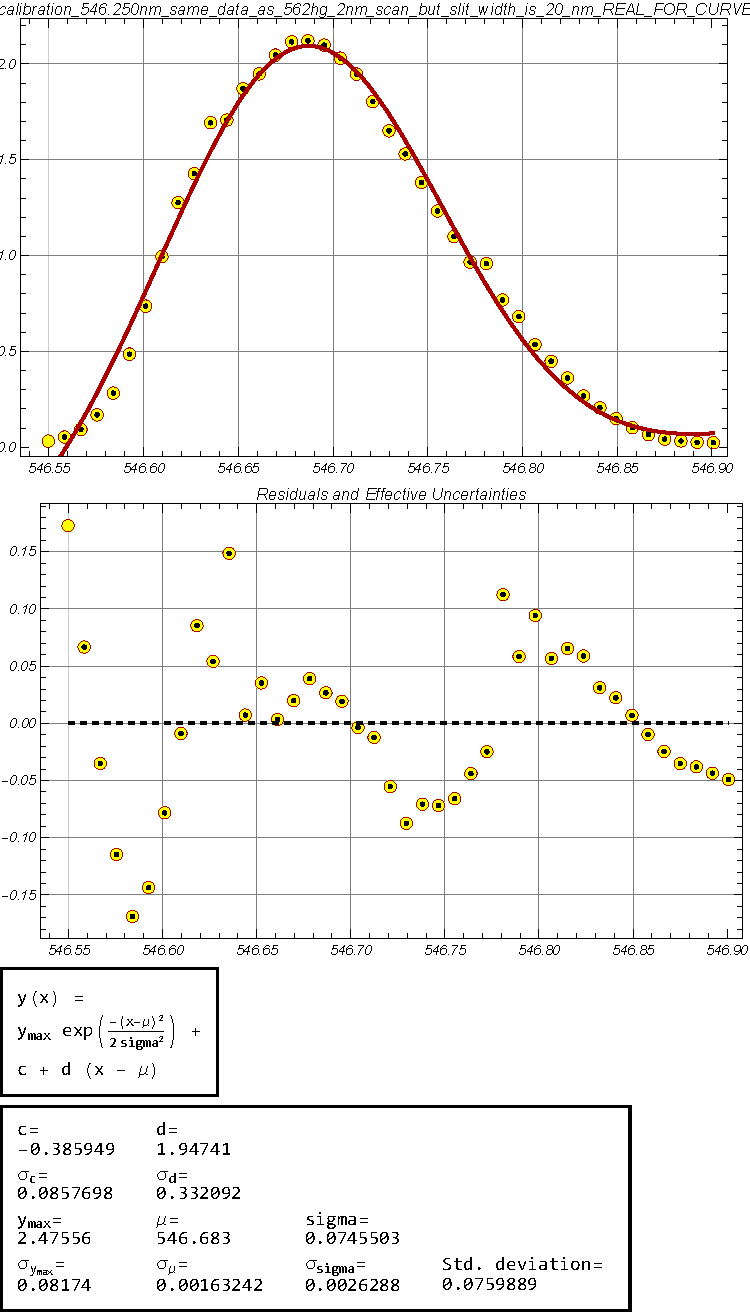
\includegraphics[width=\textwidth,height=0.78\textheight,keepaspectratio]{CurveFit_appendix/Hg_calibration_fit_reports/CF_Hg_546_repeat_20um_slit_appendix.pdf}
\caption{CurveFit repeat scan at 546 nm, 20 um slit configuration.}
\end{figure}

\end{document}